\chapter{Client} 
\label{ch:Chapter6}
\vfill \minitoc \newpage

The client was implemented in Android and uses Android's Jetpack Compose UI toolkit.

\begin{figure}[!ht]
	\centering
	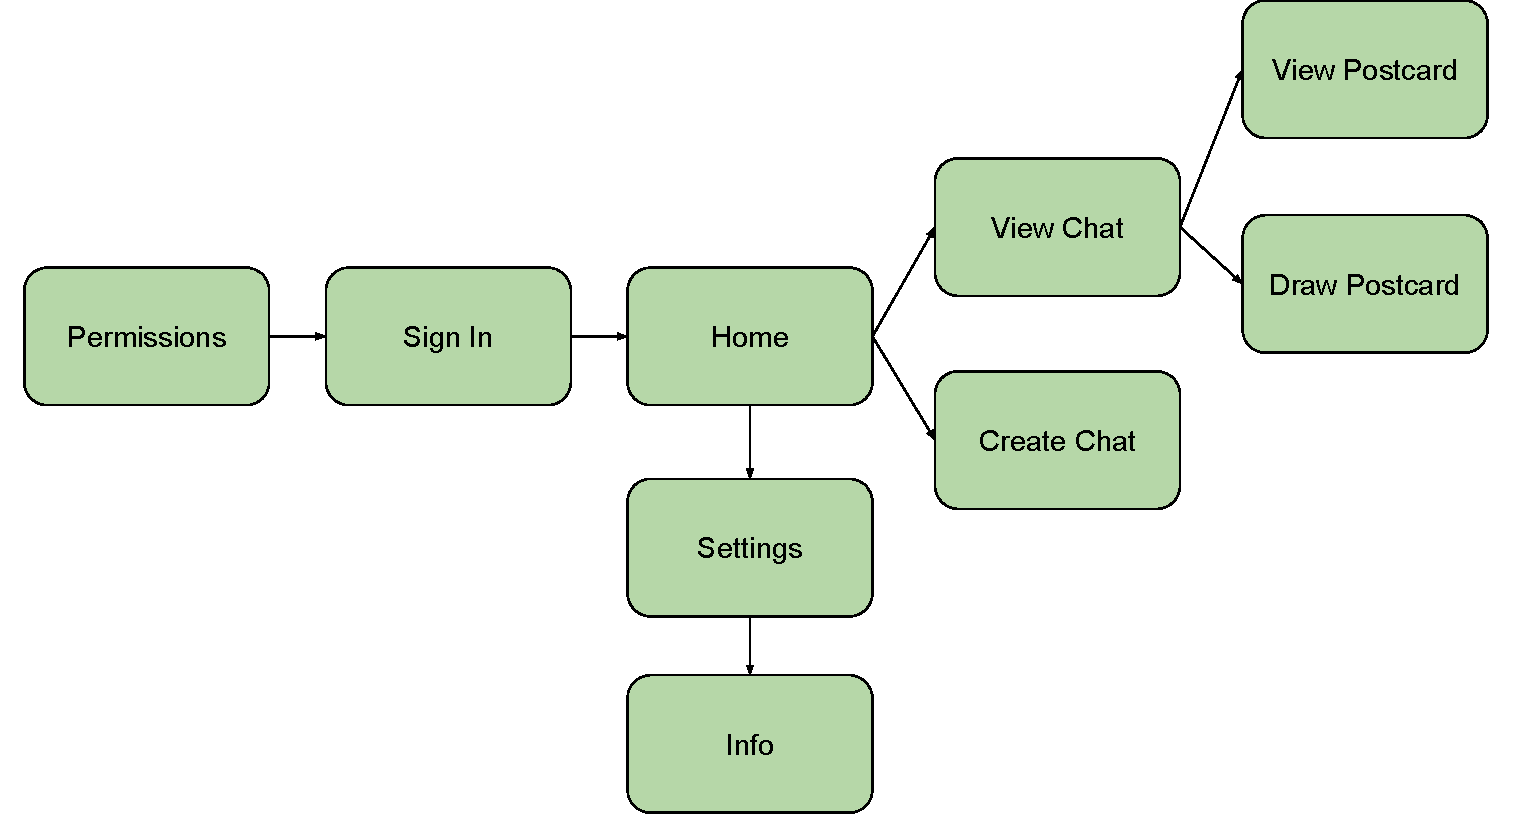
\includegraphics[trim={0cm 0cm 0 0cm}, width=1\textwidth]{./Chapter6/Figures/Android NavGraph}
	\caption{Android Activity Navigation Graphic}
	\label{fig:NavgGraph}
\end{figure}


\section{Android System and Compose Framework Overview}
Before showing the client implementation its best to give some context and basic knowledge about the android system and the Compose framework.

\subsection{Android Manifest}
The AndroidManifest.xml file is an essential configuration file in Android development that provides essential information about the Android application to the Android system. It is located in the root directory of the Android project and is required for every Android application.

The Android manifest file contains important metadata about the app, including its package name, version number, permissions, activities, services, broadcast receivers, and more. It serves as a blueprint for the Android system to understand the structure and behavior of the application.

\subsection{Android Activity}
In the context of Android app development, an Activity is a fundamental component of an Android application that represents a single screen with a user interface. It is a crucial part of the overall app architecture and is responsible for handling user interactions and presenting visual elements to the user.

An Activity acts as a container for the user interface and provides a window in which the app's UI elements, such as buttons, text fields, images, and other widgets, are displayed. It manages the lifecycle of these UI components and handles user input events, such as button clicks or touch gestures.

Each Activity has a corresponding Java or Kotlin class that extends the Activity base class or its subclasses provided by the Android framework. This class contains methods that define the behavior of the Activity during different stages of its lifecycle, such as creation, starting, pausing, resuming, stopping, and destruction.

When an app is launched, typically, the main Activity is created and displayed to the user. The Activity is responsible for setting up the initial UI layout, interacting with data sources (e.g., retrieving data from a database or an API), and responding to user actions. It can also communicate with other Activities, such as starting a new Activity for a different screen or receiving results from a previously started Activity.

\subsection{Data Storing}
Android uses a file system that's similar to disk-based file systems on other platforms. The system provides several options for you to save your app data:
\begin{itemize}
    \item App-specific storage: Store files that are meant for your app's use only, either in dedicated directories within an internal storage volume or different dedicated directories within external storage. Use the directories within internal storage to save sensitive information that other apps shouldn't access;
    \item Shared storage: Store files that your app intends to share with other apps, including media, documents, and other files;
    \item Preferences: Store private, primitive data in key-value pairs;
    \item Databases: Store structured data in a private database using the Room persistence library.    
\end{itemize}


\subsection{ViewModel}
The ViewModel class is a business logic or screen level state holder. It exposes state to the UI and encapsulates related business logic. Its principal advantage is that it caches state and persists it through configuration changes. This means that your UI doesn’t have to fetch data again when navigating between activities, or following configuration changes, such as when rotating the screen.

\subsection{Canvas}
The Android Canvas is a fundamental graphics component provided by the Android framework. It serves as a drawing surface onto which we can render custom graphics, shapes, images, and text. The Canvas provides a set of drawing methods that allow us to create and manipulate visual elements within an Android application.

When working with the Canvas, we can perform various operations such as drawing lines, rectangles, circles, arcs, and paths. We can also apply transformations like translation, rotation, scaling, and skewing to manipulate the position and orientation of the drawn elements. Additionally, the Canvas supports the rendering of text, allowing us to display custom text with different fonts, sizes, colors, and styles.

\subsection{Making HTTP Request}
When developing Android applications, it is common to interact with web services and APIs to retrieve data or send data to a server. One popular library for making HTTP requests in Android is OkHttp.

\subsubsection{OkHttp}
OkHttp is an open-source HTTP client library for Java and Android applications. It is developed by the same team behind the widely-used Retrofit library and offers a simple and efficient way to make HTTP requests and handle responses. OkHttp is built on top of the Java standard library's HttpURLConnection, providing a more convenient and powerful API.


\section{Activities}
In this section we will demonstrate all activities implemented.
\subsection{Permissions}
The Permissions activity handles all requests to permissions needed for the application to work.
The Application needs permission to read contacts.

Figures \ref{fig:PA} illustrates the implemented activity. 

\begin{figure}[!ht]
	\centering
	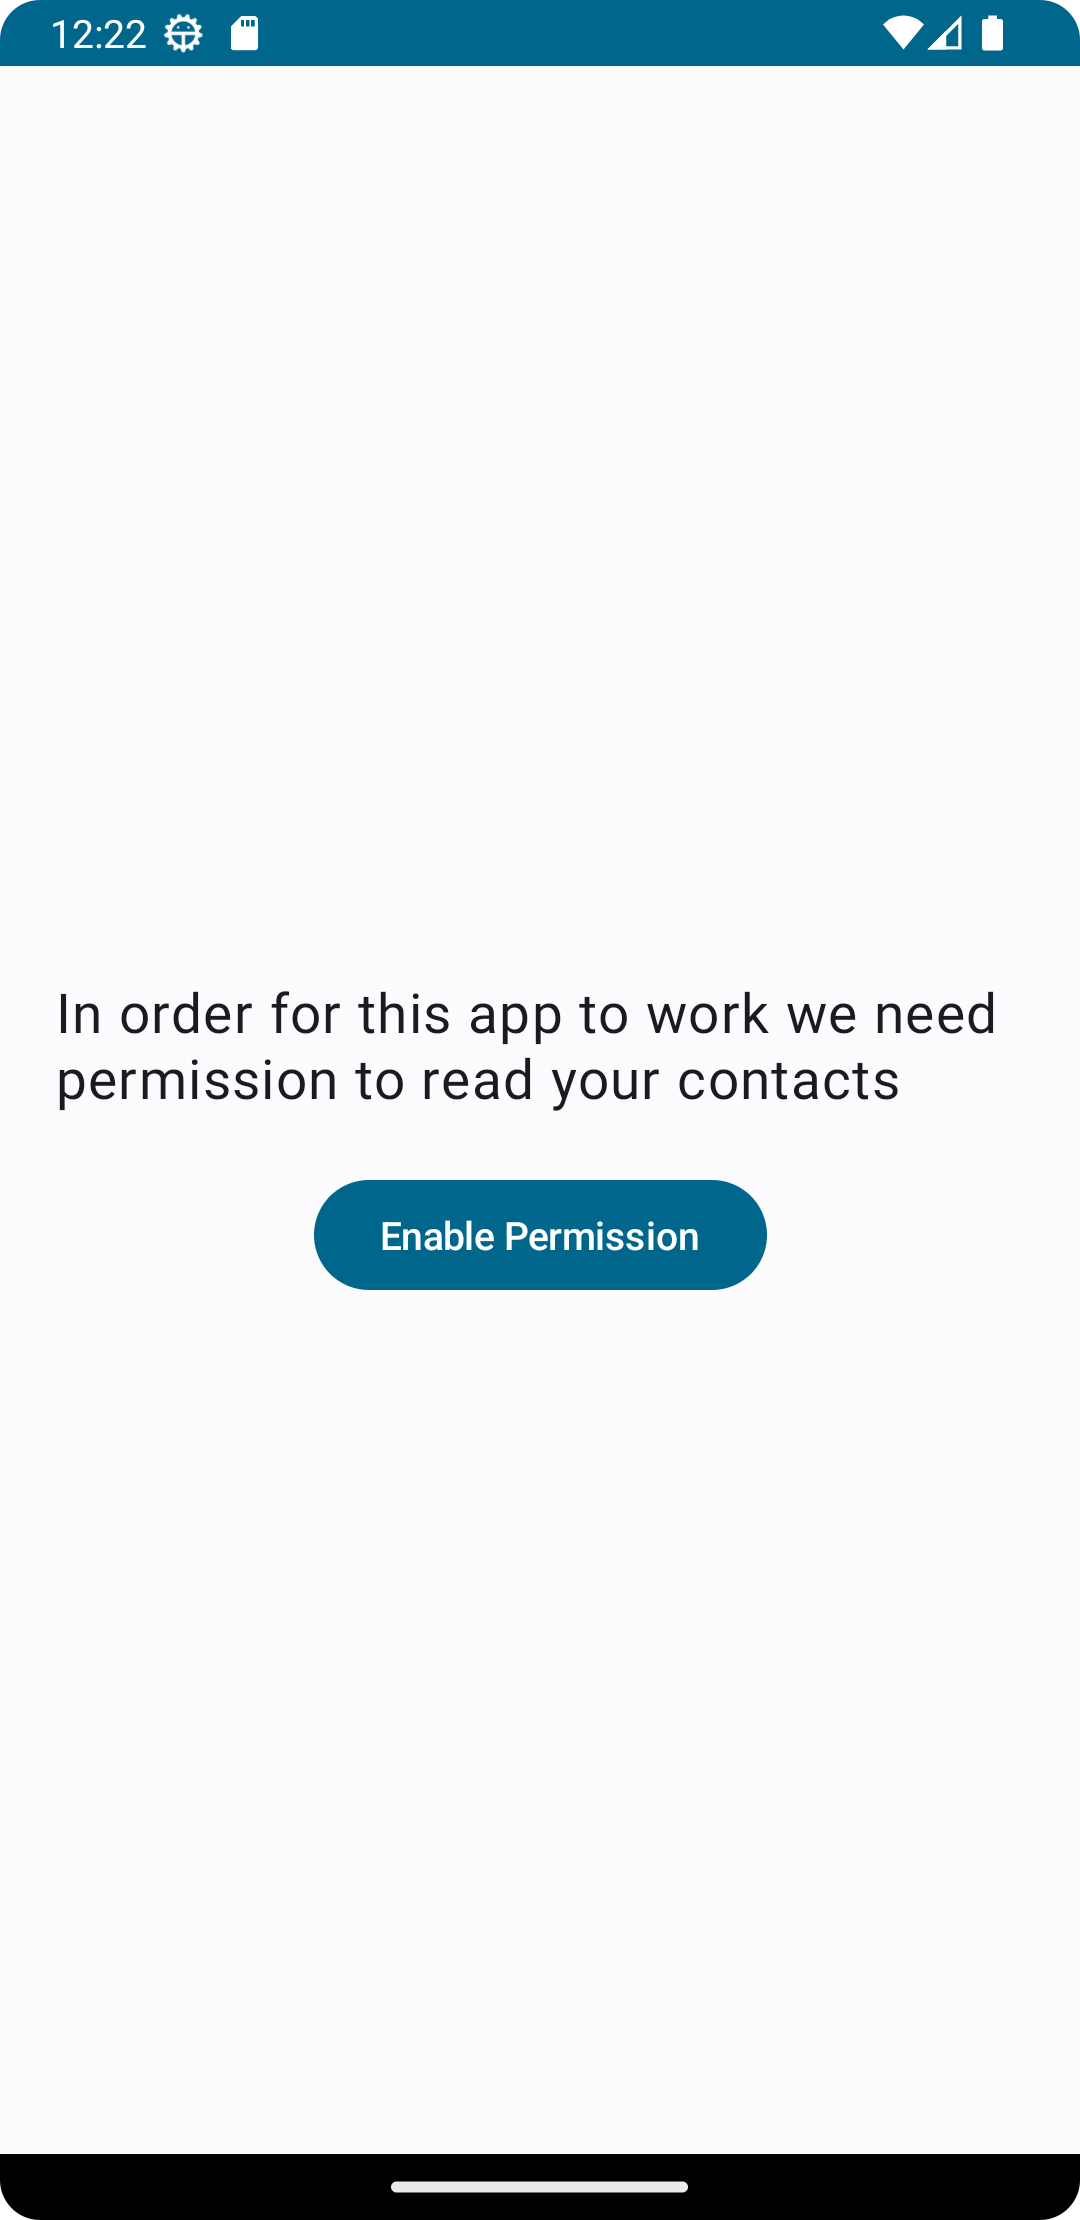
\includegraphics[trim={0cm 0cm 0 0cm}, width=0.4\textwidth]{./Chapter6/Figures/PermissionActivity}
	\caption{Permission Activity}
	\label{fig:PA}
\end{figure}


\subsection{Sign In}

The Sign-in Activity serves as the component for managing the user's authentication process, containing both logging in and registering in the service. Additionally, it ensures the secure storage of the user's token by leveraging the EncryptedSharedPreferences.

Upon launching the Sign-in Activity, users are presented with a user-friendly interface where they can enter their credentials or choose to register as a new user. The activity handles the input validation and securely communicates with the server-side authentication API.

Once the user's credentials are verified, the Sign-in Activity retrieves the authentication token from the server's response. To ensure the token's confidentiality, it is stored using the EncryptedSharedPreferences. This specialized SharedPreferences implementation employs encryption algorithms to protect sensitive data from unauthorized access.

By utilizing the EncryptedSharedPreferences, the Sign-in Activity safeguards the user's authentication token, preventing it from being tampered with or exposed. This secure storage mechanism provides an additional layer of protection for user data, mitigating the risks associated with unauthorized token access.


In addition, the Sign-in Activity incorporates an automatic phone number region retrieval feature by leveraging the Carrier information.

Because our app hasn't been deployed anywhere it is prompted to the user to choose whether he wants to use local data "Mock" or connect to an IP address - see \ref{SAIP}

Figures \ref{fig:SA1}, \ref{fig:SA2} illustrate the implemented activity.

\begin{figure}[!ht]
	\centering
	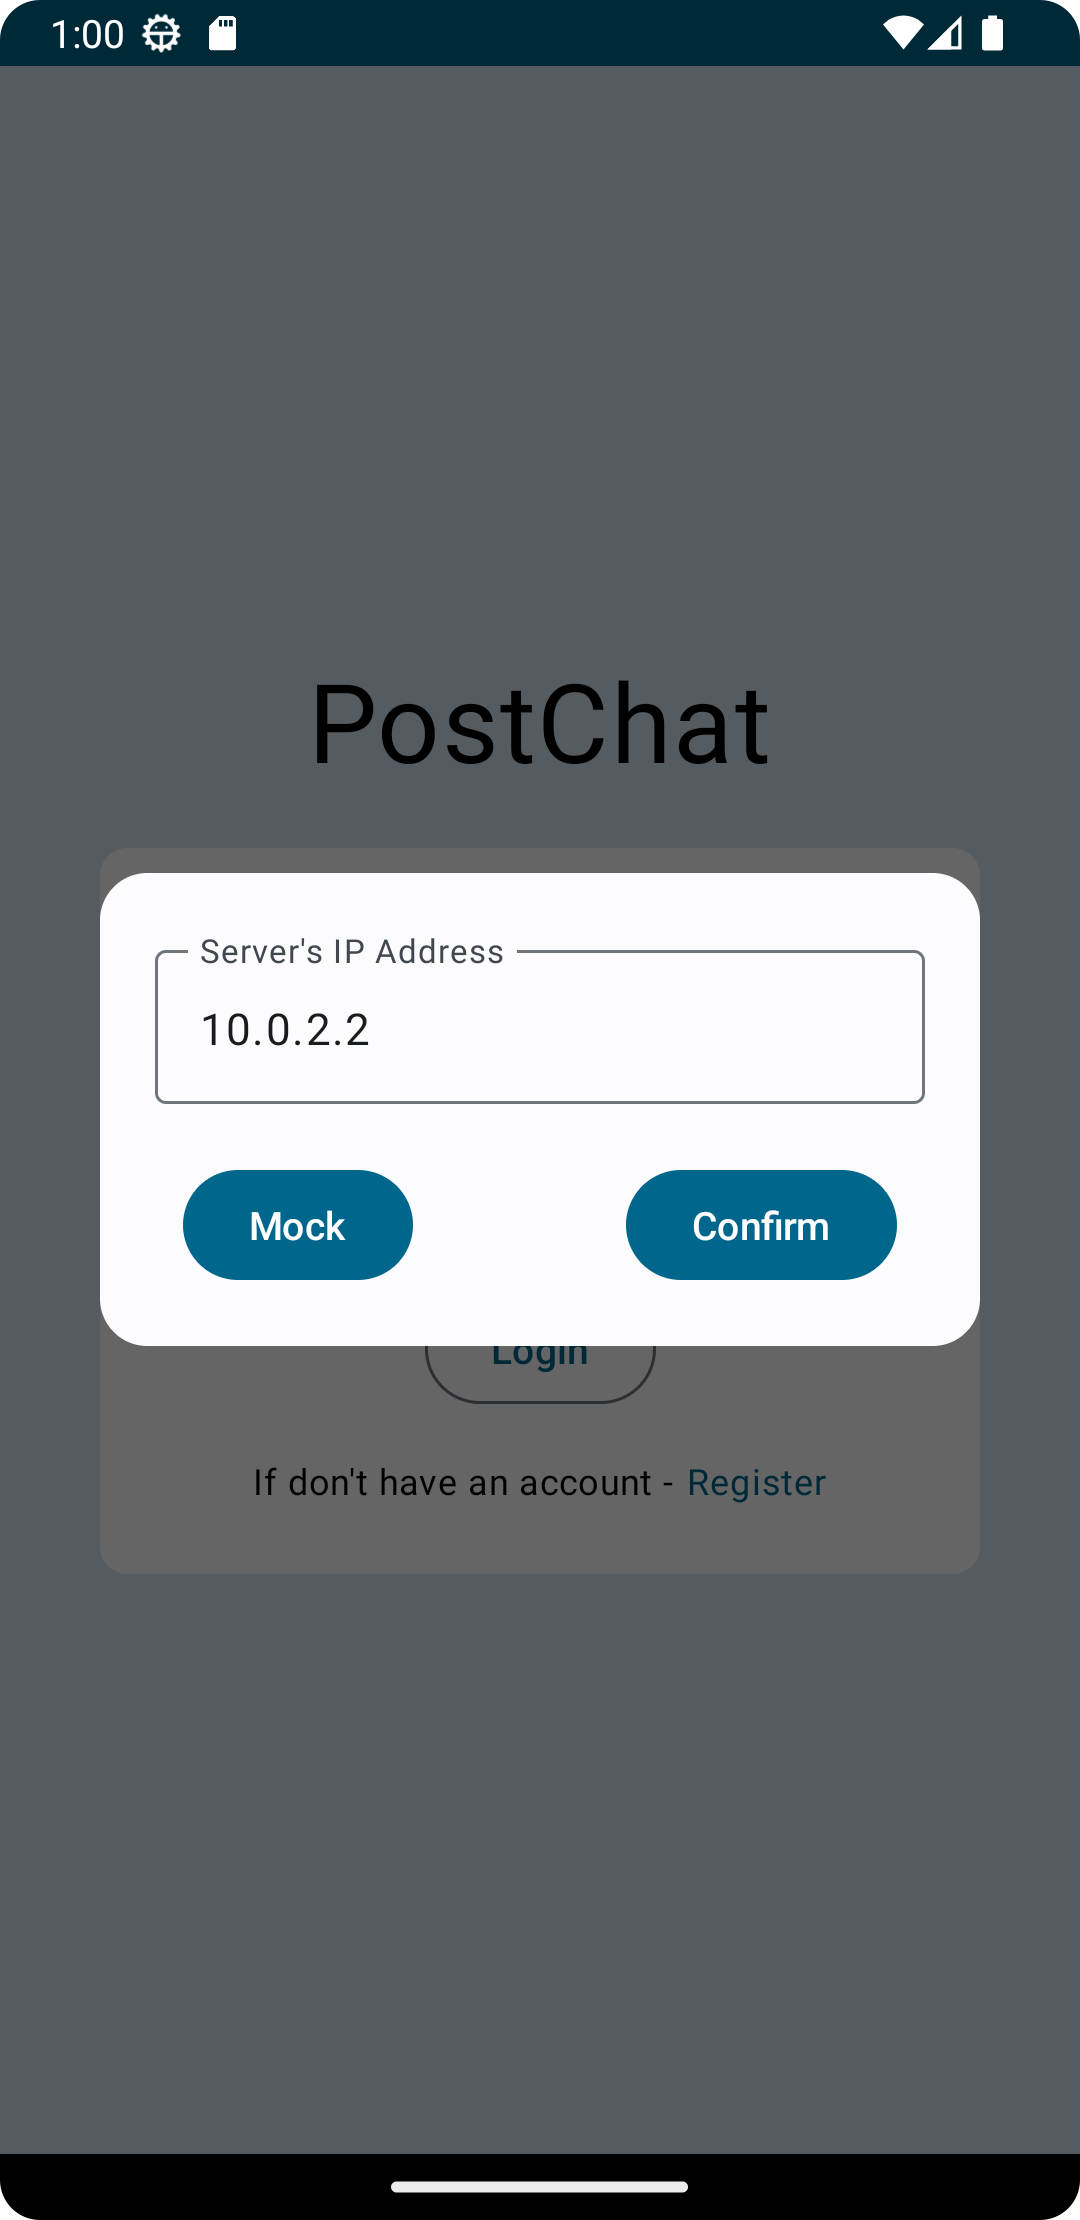
\includegraphics[trim={0cm -3cm 0 -3cm}, width=0.4\textwidth]{./Chapter6/Figures/SignInActivityIpAdress}
	\caption{Signin Activity}
	\label{fig:SAIP}
\end{figure}


\begin{figure}[!ht]
	\centering
	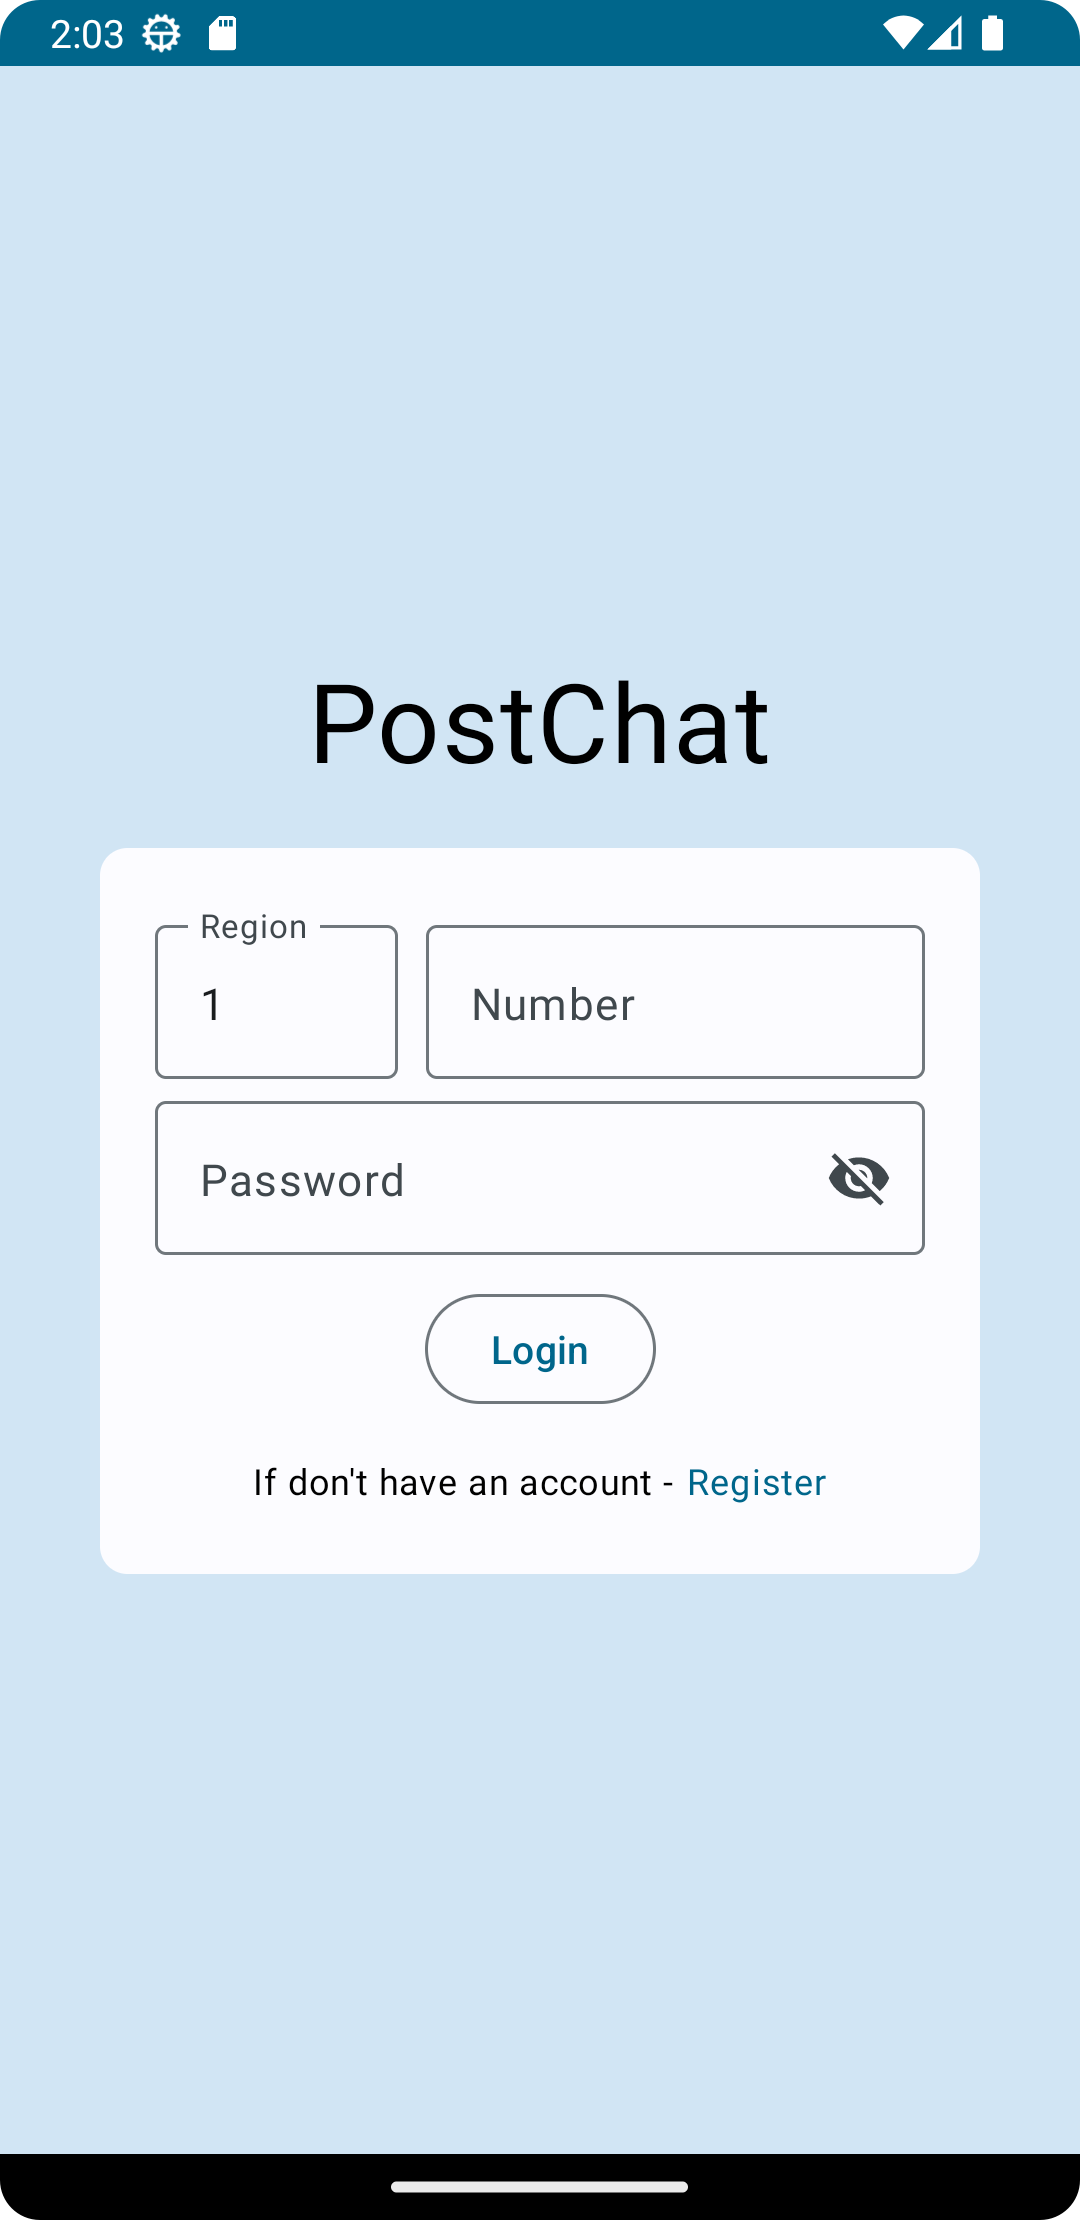
\includegraphics[trim={0cm -3cm 0 -3cm}, width=0.4\textwidth]{./Chapter6/Figures/SignInActivityLogin}
	\caption{Signin Activity}
	\label{fig:SA1}
\end{figure}


It also does local verification's to user's input. Password and Phone Number validations are done using Google's API.

\begin{figure}[!ht]
	\centering
	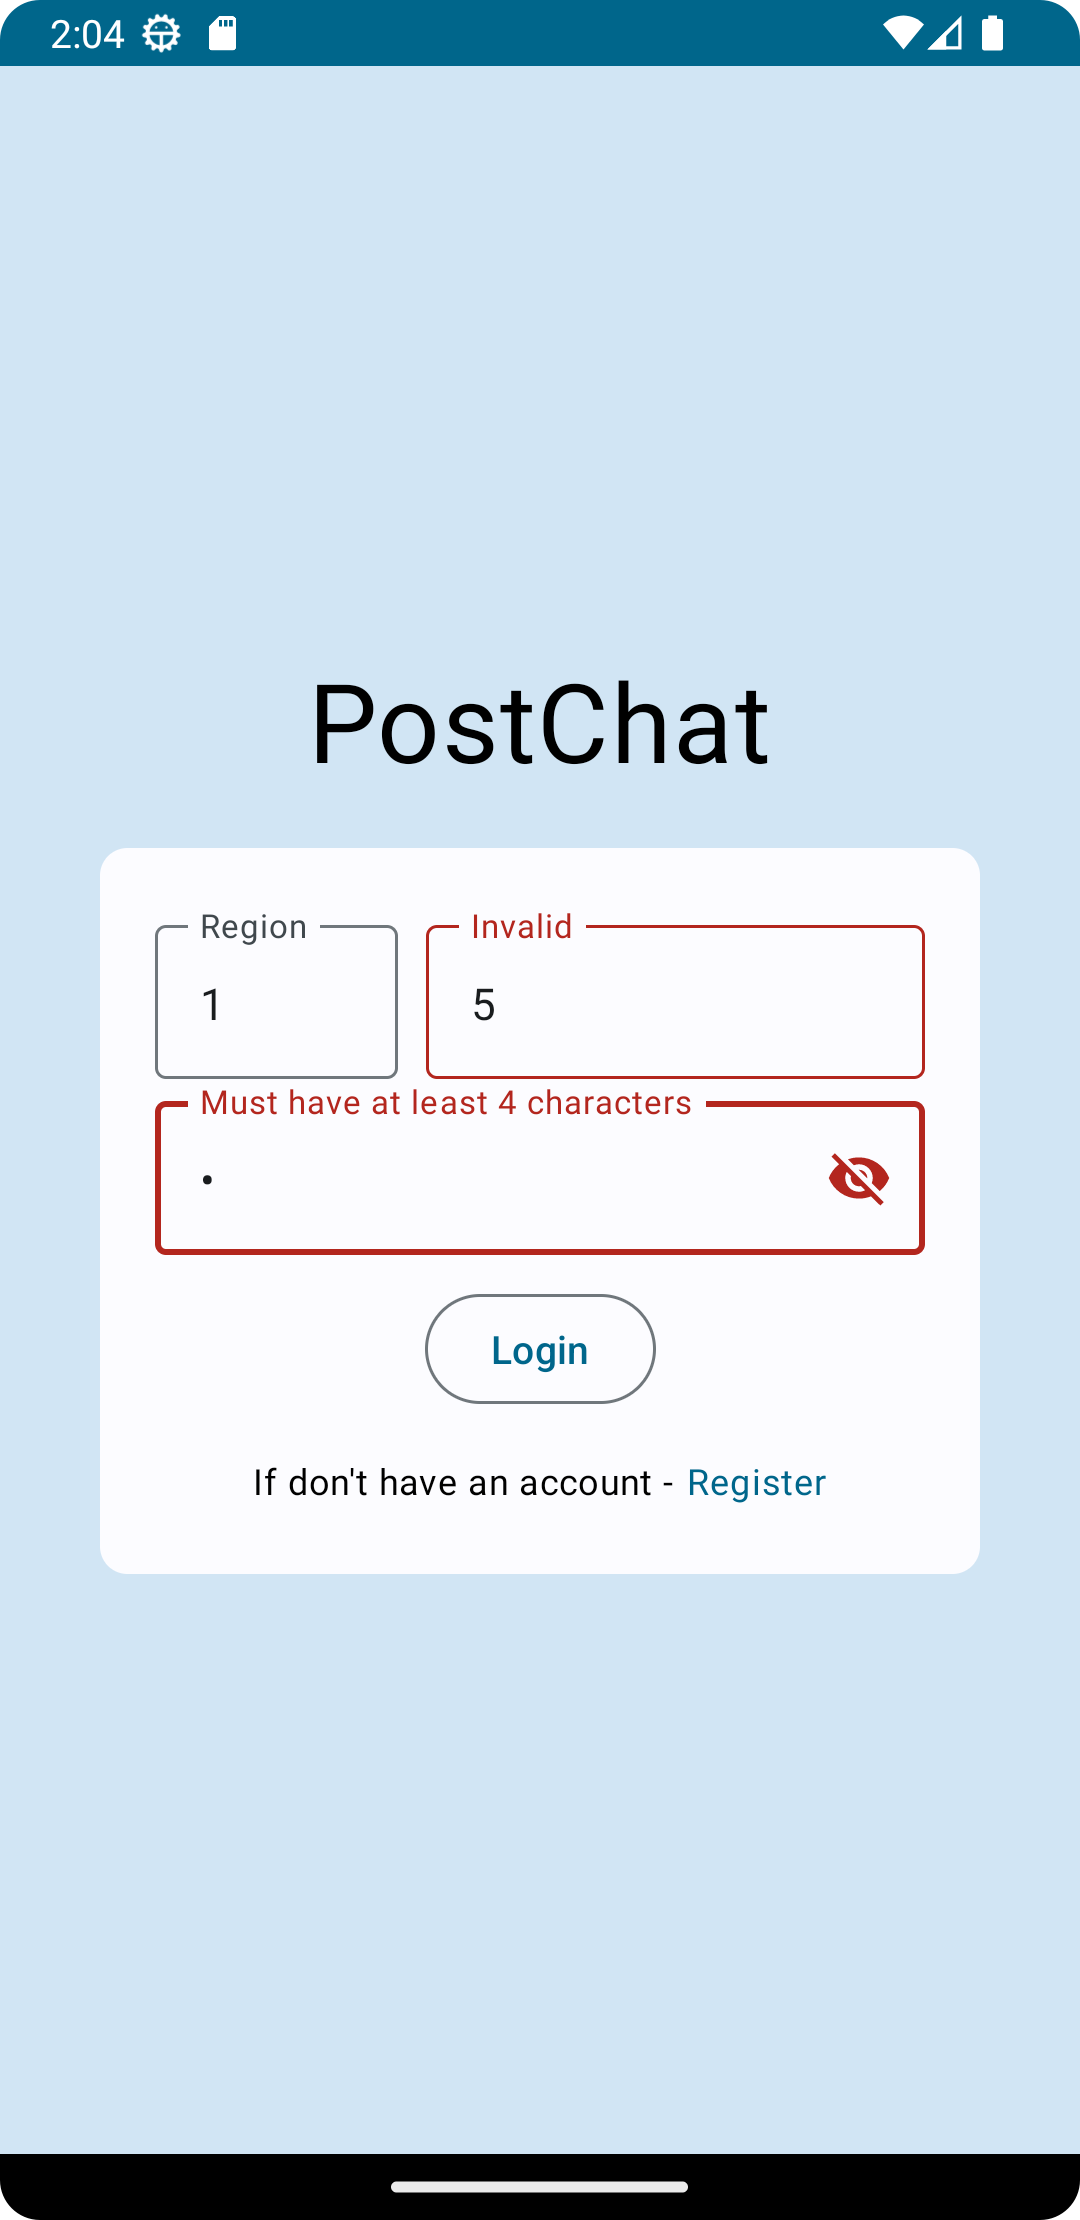
\includegraphics[trim={0cm -3cm 0 -3cm}, width=0.4\textwidth]{./Chapter6/Figures/SignInActivityErrors}
	\caption{Signin Activity invalid password size}
	\label{fig:SA2}
\end{figure}


\subsection{Home}
The Home Activity serves as a central hub for connecting to the web API and retrieving essential information related to registered users, messages, and chats. Its primary purpose is to display all chats in a user-friendly manner, with the chats ordered based on the most recent message received.

By establishing a connection with the web API, the Home Activity can fetch the necessary data to populate the chat interface. It retrieves information about registered users, ensuring that the appropriate user profiles are displayed within the chat list. Additionally, it retrieves messages associated with each chat, allowing users to view their conversation history.

The Home Activity organizes the chats in a manner that prioritizes the most recent interactions. By ordering the chats based on the last message received, users can quickly identify and access their most recent conversations.

Moreover, the Home Activity provides intuitive controls and a simple interface, users can create new chat groups, within a button.

Figure~\ref{fig:HA1} illustrate the implemented activity.

\begin{figure}[!ht]
	\centering
	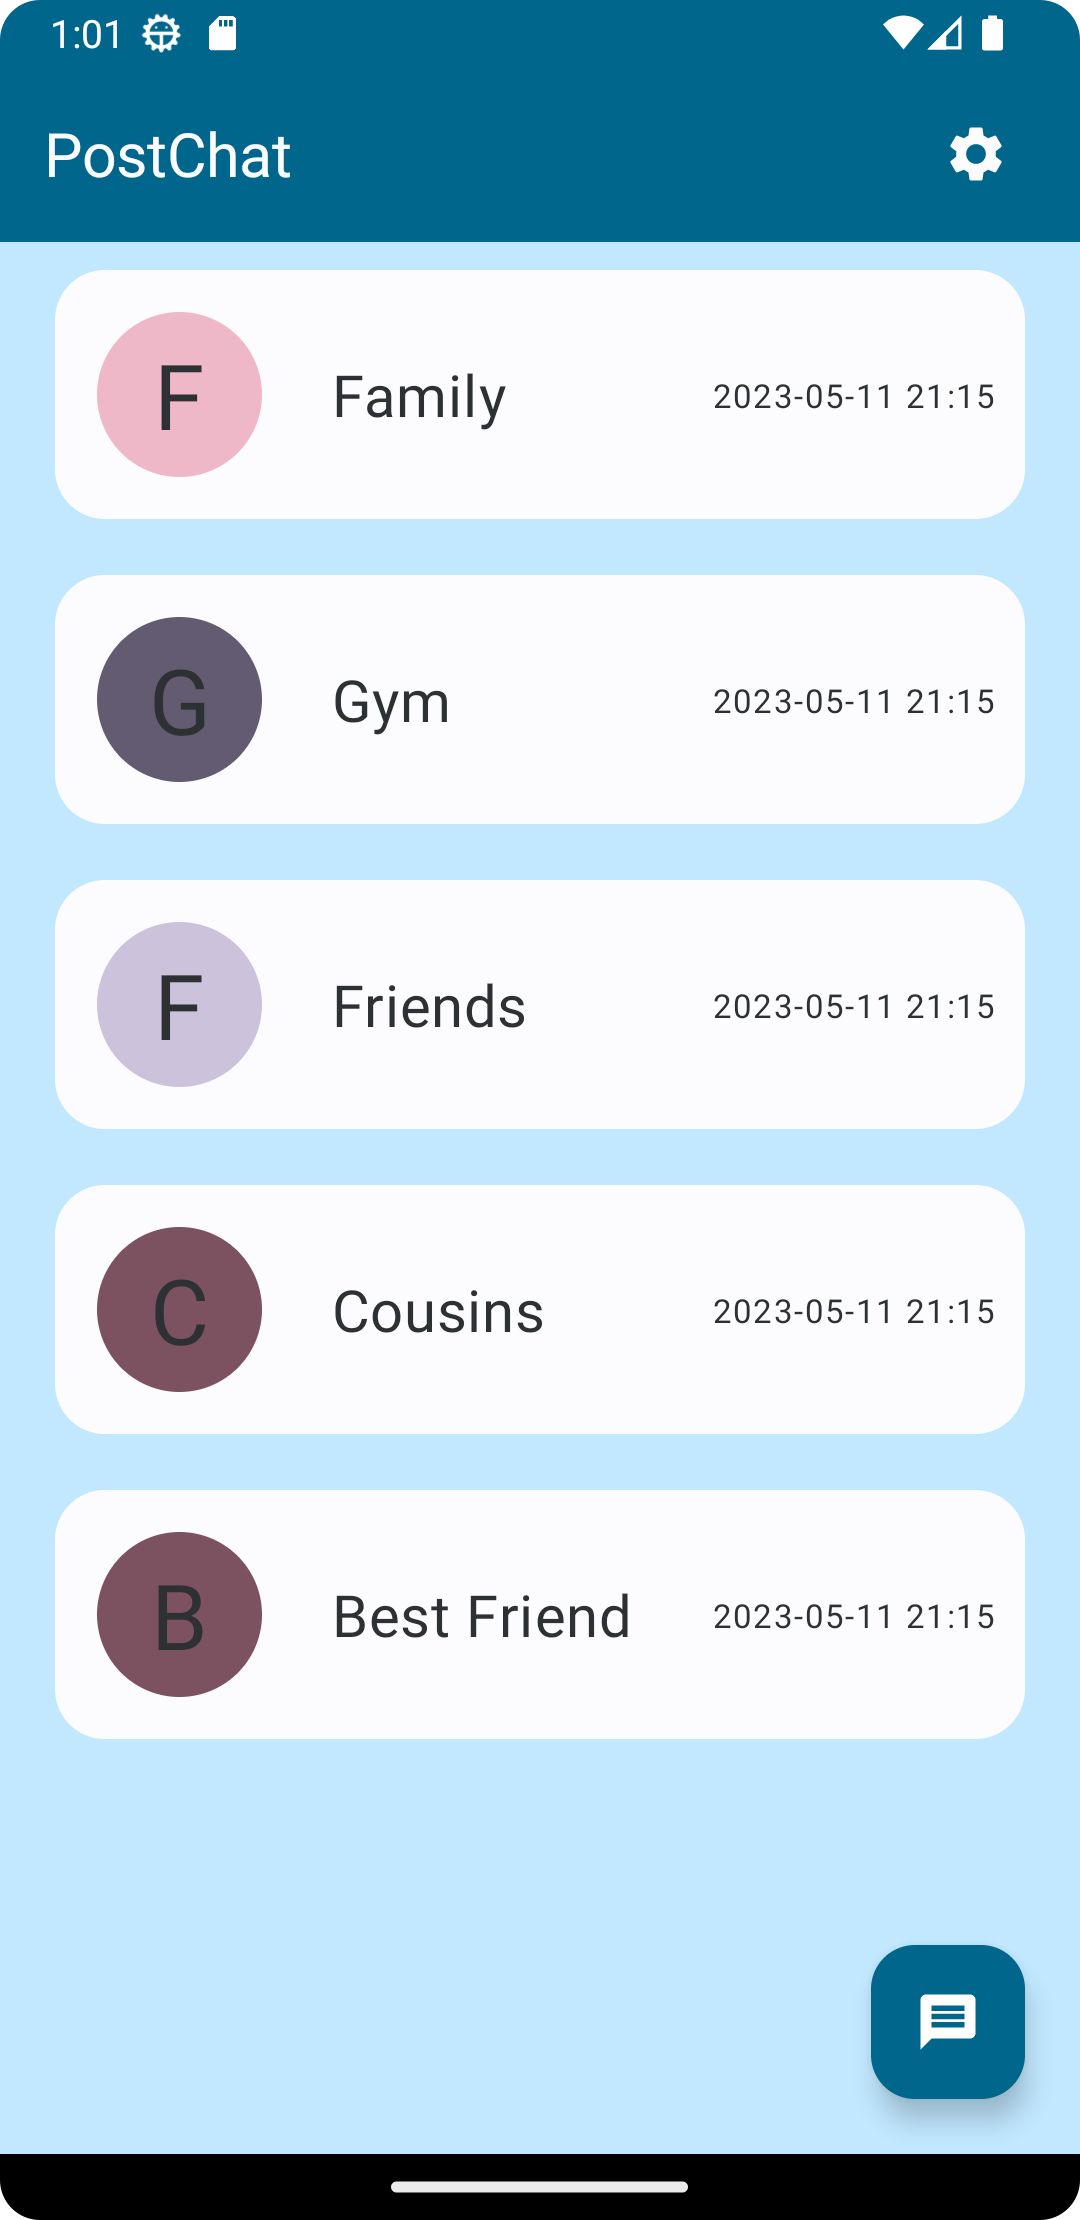
\includegraphics[trim={0cm -3cm 0 -3cm}, width=0.4\textwidth]{./Chapter6/Figures/HomeActivity}
	\caption{Home Activity}
	\label{fig:HA1}
\end{figure}


\subsection{Create Chat}
The CreateChat activity searches for the users stored in the local database and lets you pick the phone numbers you want to add to the chat. Every chat needs a name so a popup dialog input message shows when clicking the check button.

Figures \ref{fig:CCA1} and \ref{fig:CCA2} illustrate the implemented activity.


\begin{figure}[!ht]
	\centering
	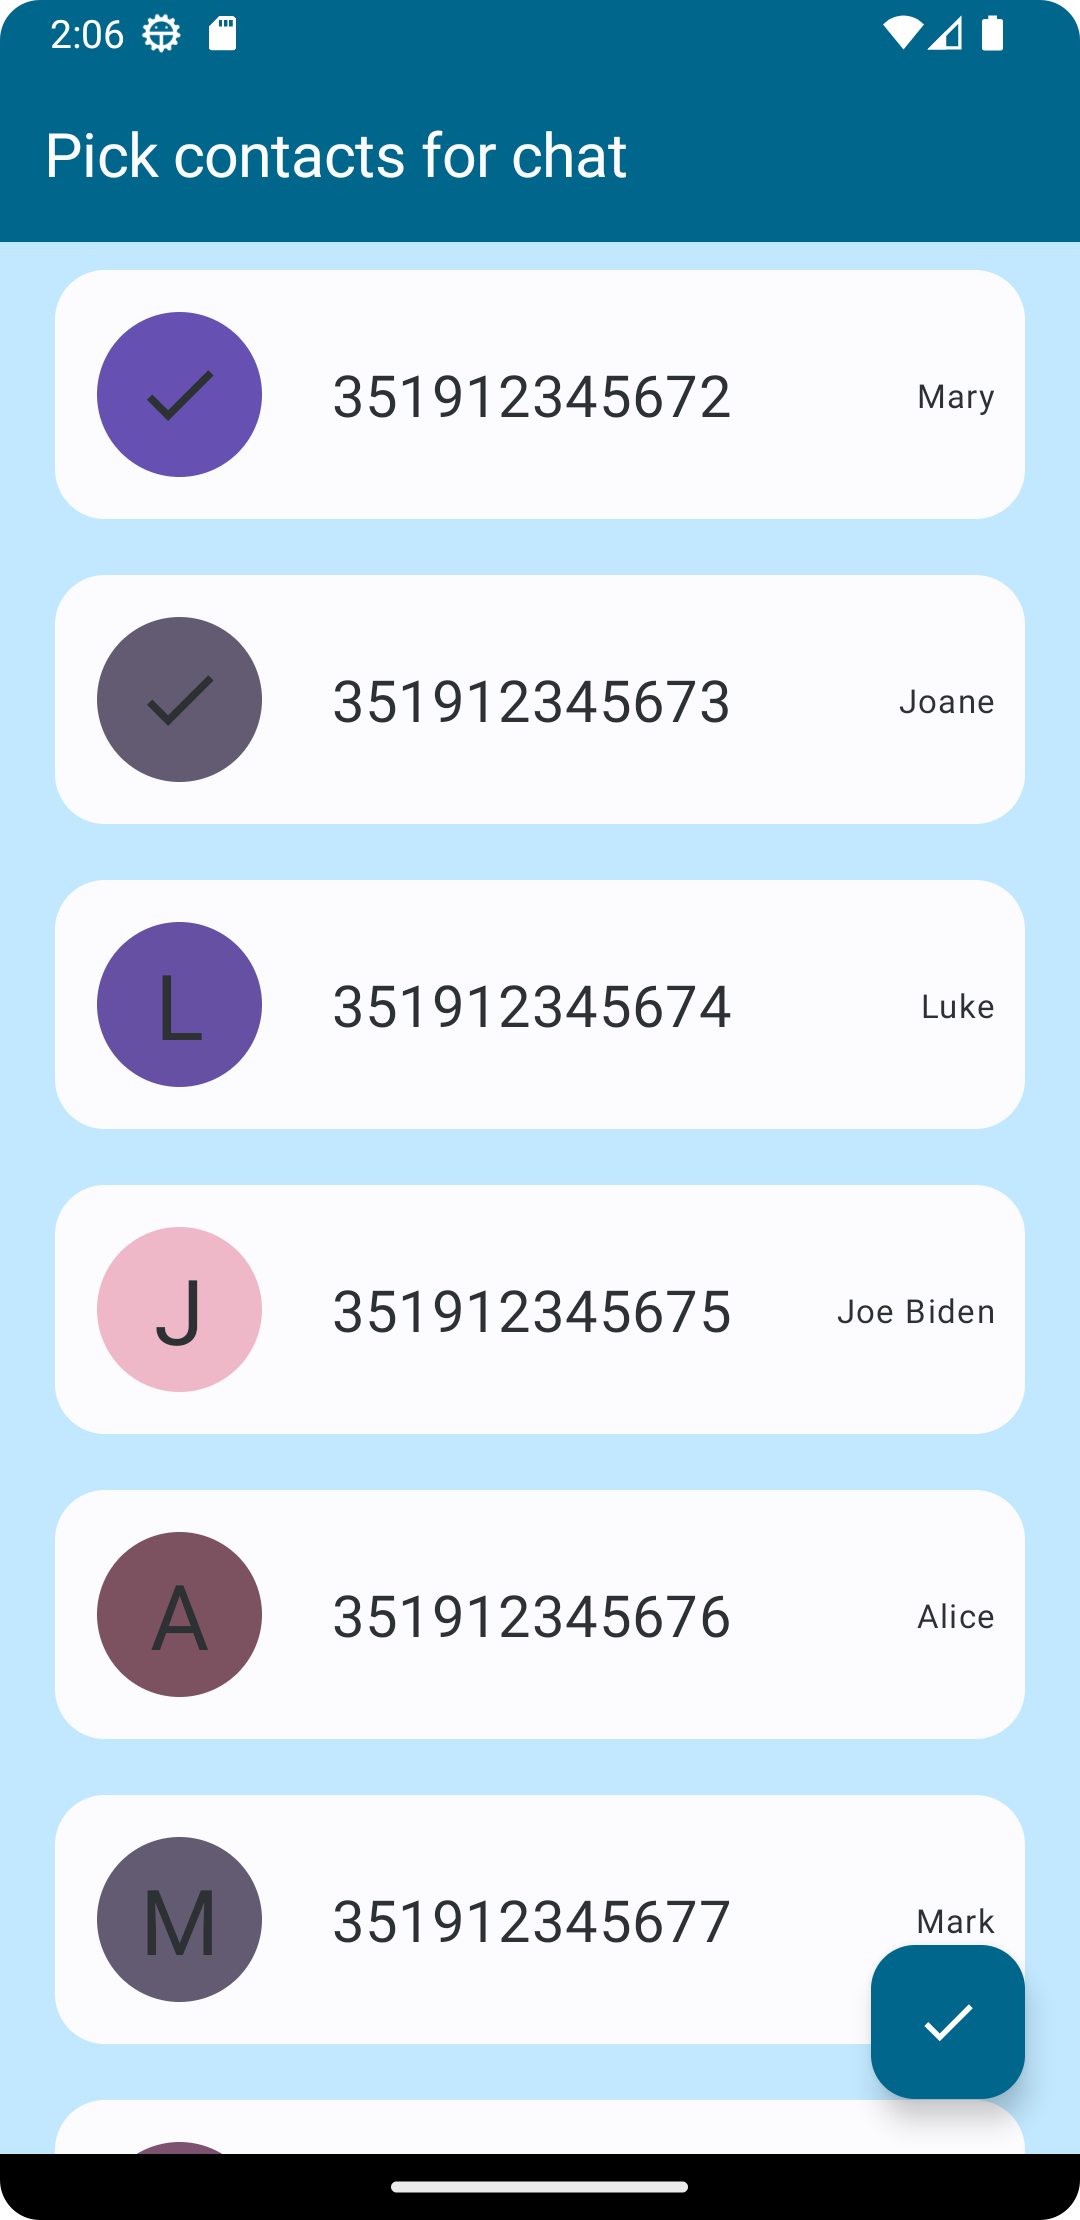
\includegraphics[trim={0cm -3cm 0 -3cm}, width=0.4\textwidth]{./Chapter6/Figures/CreateChatActivityPickContacts}
	\caption{CreateChat Activity}
	\label{fig:CCA1}
\end{figure}


\begin{figure}[!ht]
	\centering
	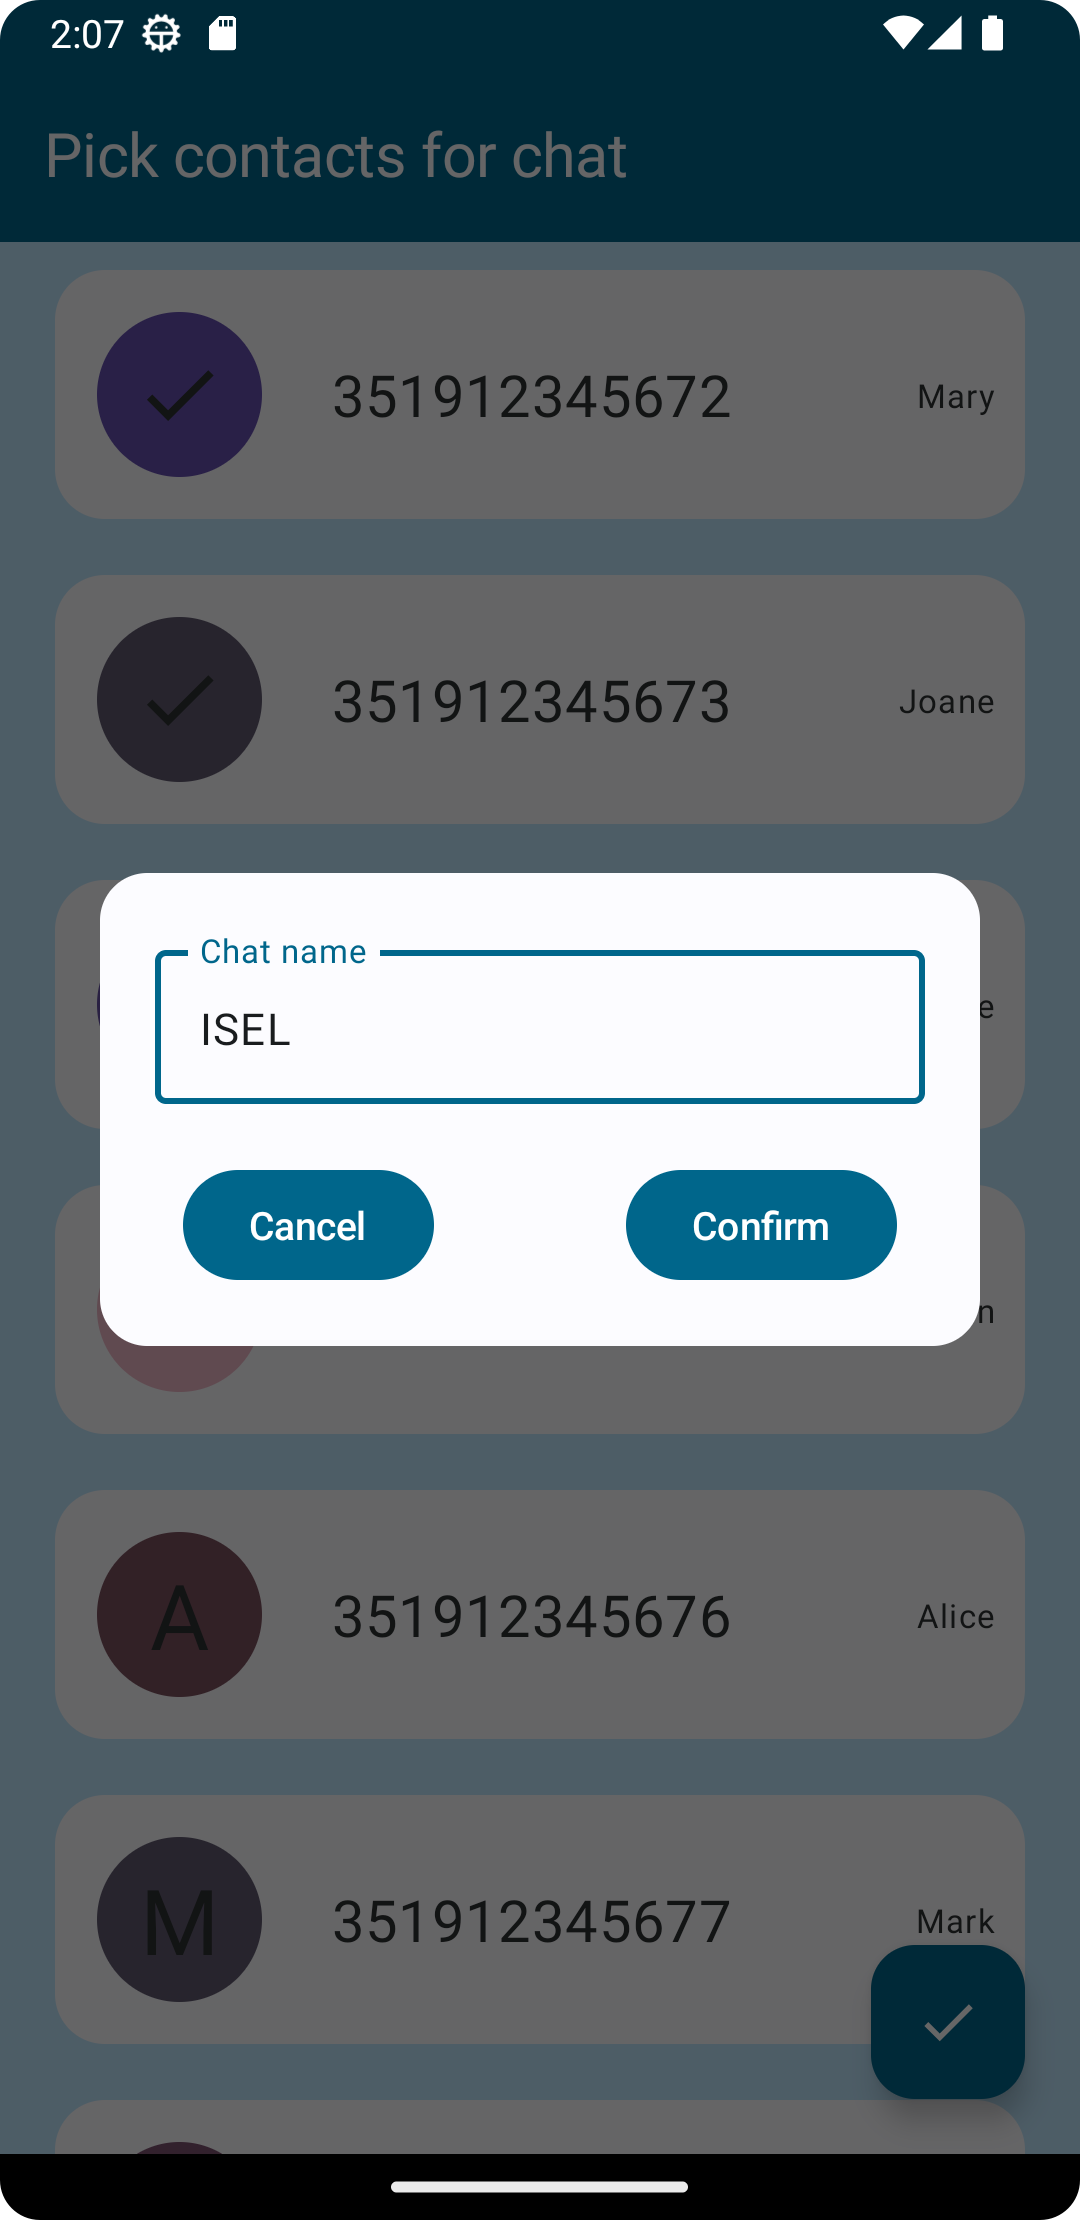
\includegraphics[trim={0cm -3cm 0 -3cm}, width=0.4\textwidth]{./Chapter6/Figures/CreateChatActivityName}
	\caption{CreateChat Activity name prompt}
	\label{fig:CCA2}
\end{figure}

\subsection{Chat View}
The Chat activity obtains the information about the current chat messages. 
It displays the postcards in order by the timestamp and above the same it shows the number from the person that sent the message. In the future this will be changed to query users in the local database and get their name.  

Figures \ref{fig:CVA1}, \ref{fig:CVA2} , \ref{fig:CVA3} and \ref{fig:CVA4} illustrate the implemented activity.

\begin{figure}[!ht]
	\centering
	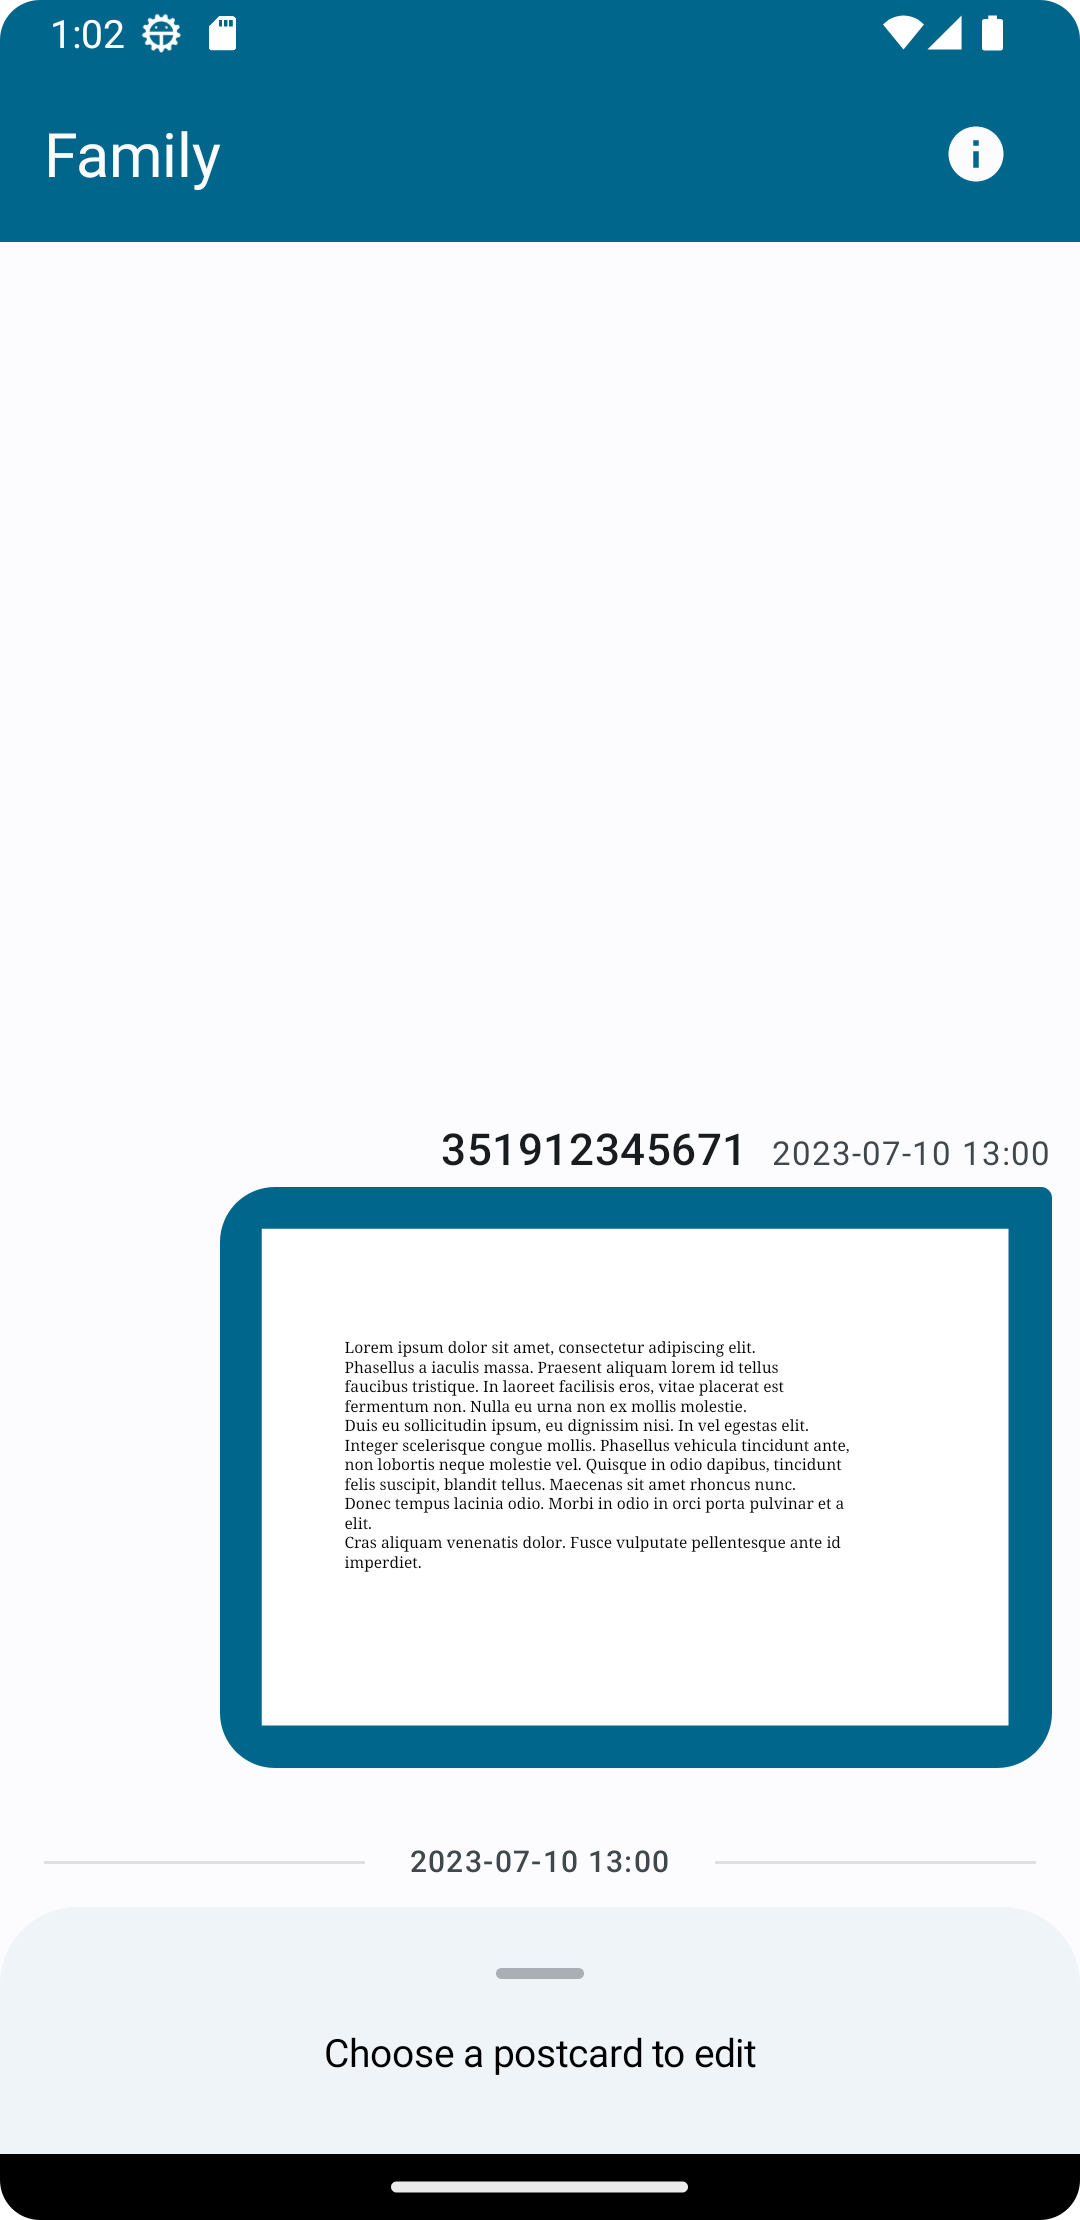
\includegraphics[trim={0cm -3cm 0 -3cm}, width=0.4\textwidth]{./Chapter6/Figures/ChatActivity}
	\caption{Chat Activity}
	\label{fig:CVA1}
\end{figure}


\begin{figure}[!ht]
	\centering
	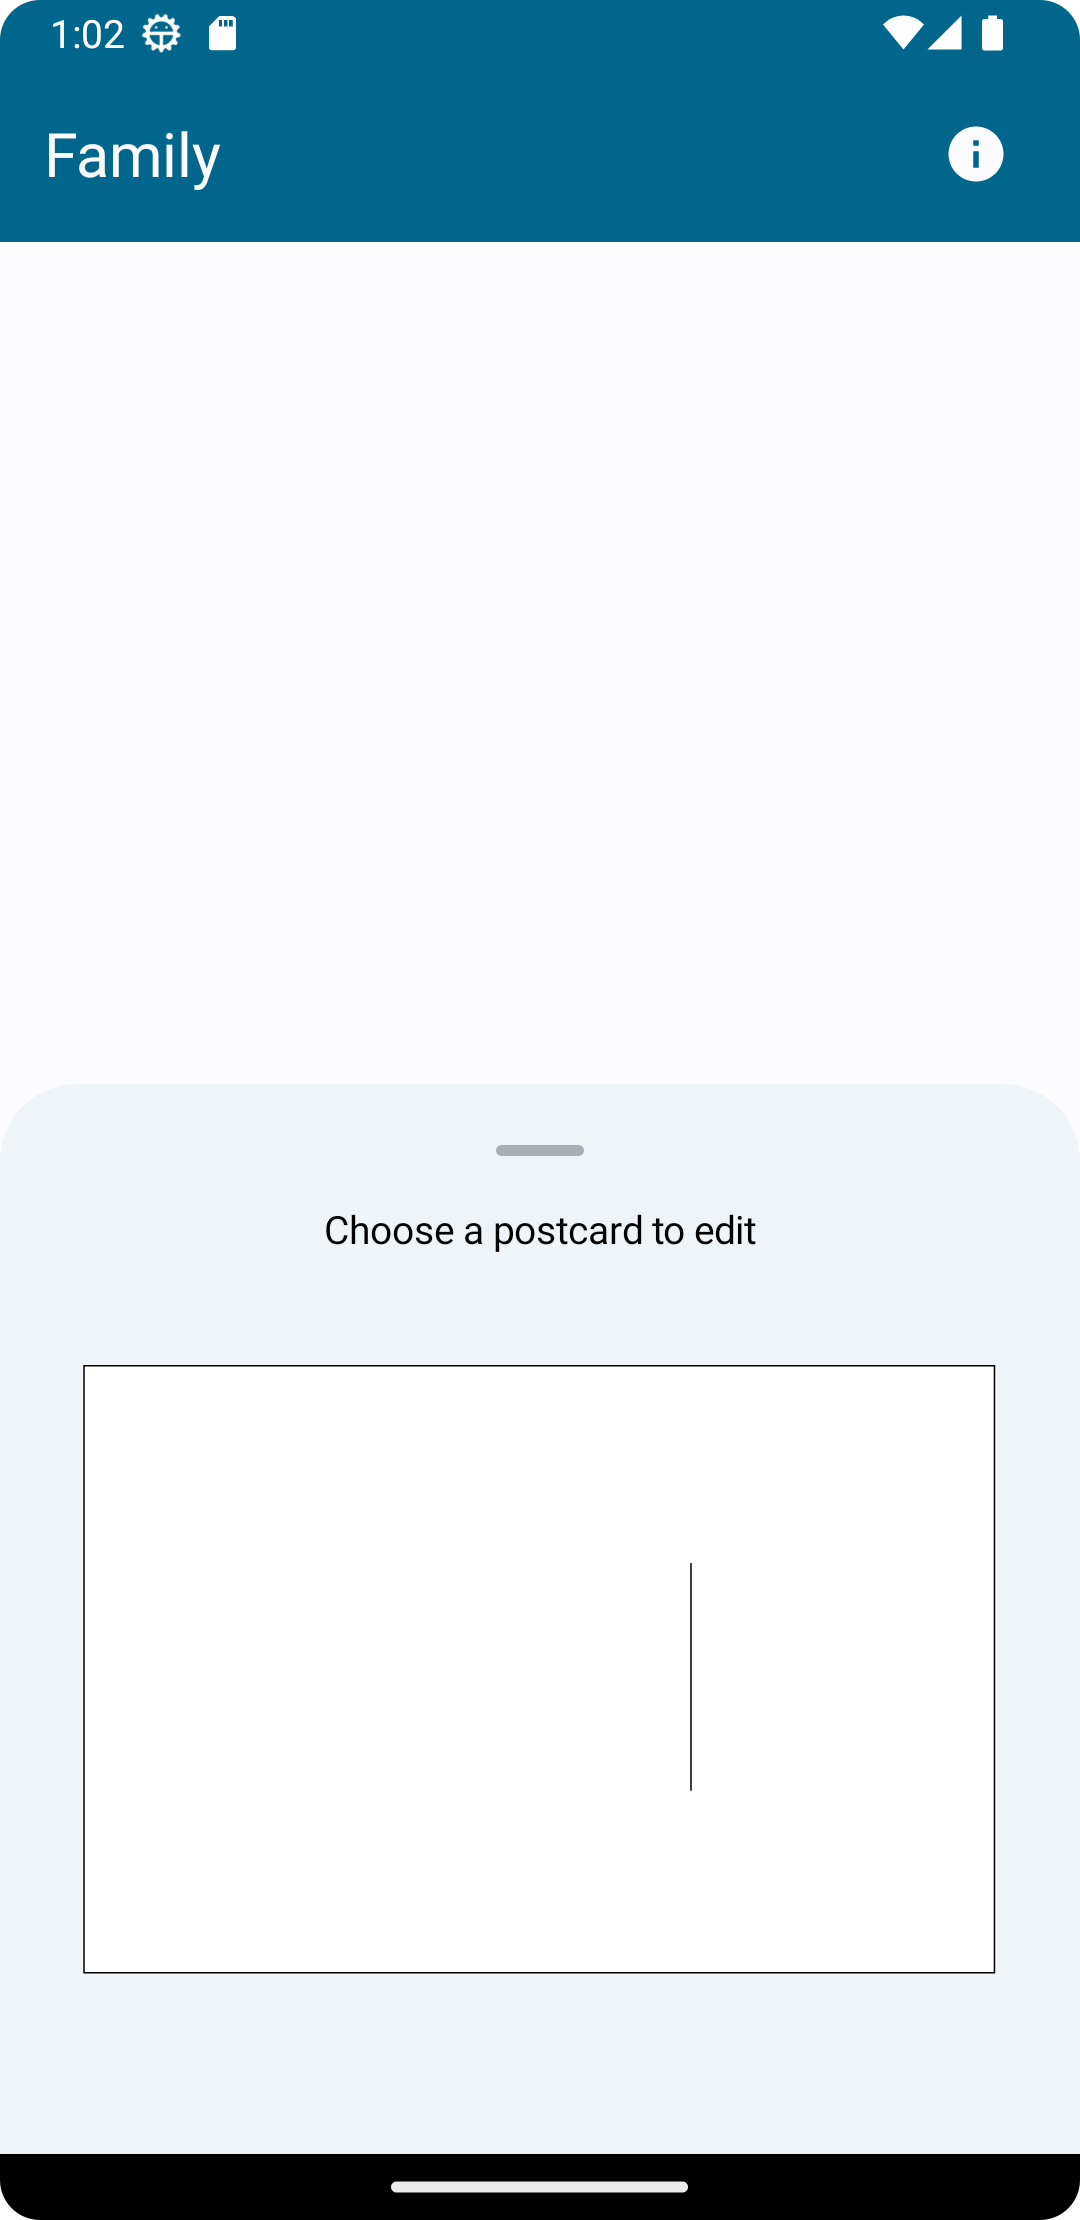
\includegraphics[trim={0cm -3cm 0 -3cm}, width=0.4\textwidth]{./Chapter6/Figures/ChatActivityShowPostcards}
	\caption{Chat Activity bottom templates list}
	\label{fig:CVA2}
\end{figure}


\begin{figure}[!ht]
	\centering
	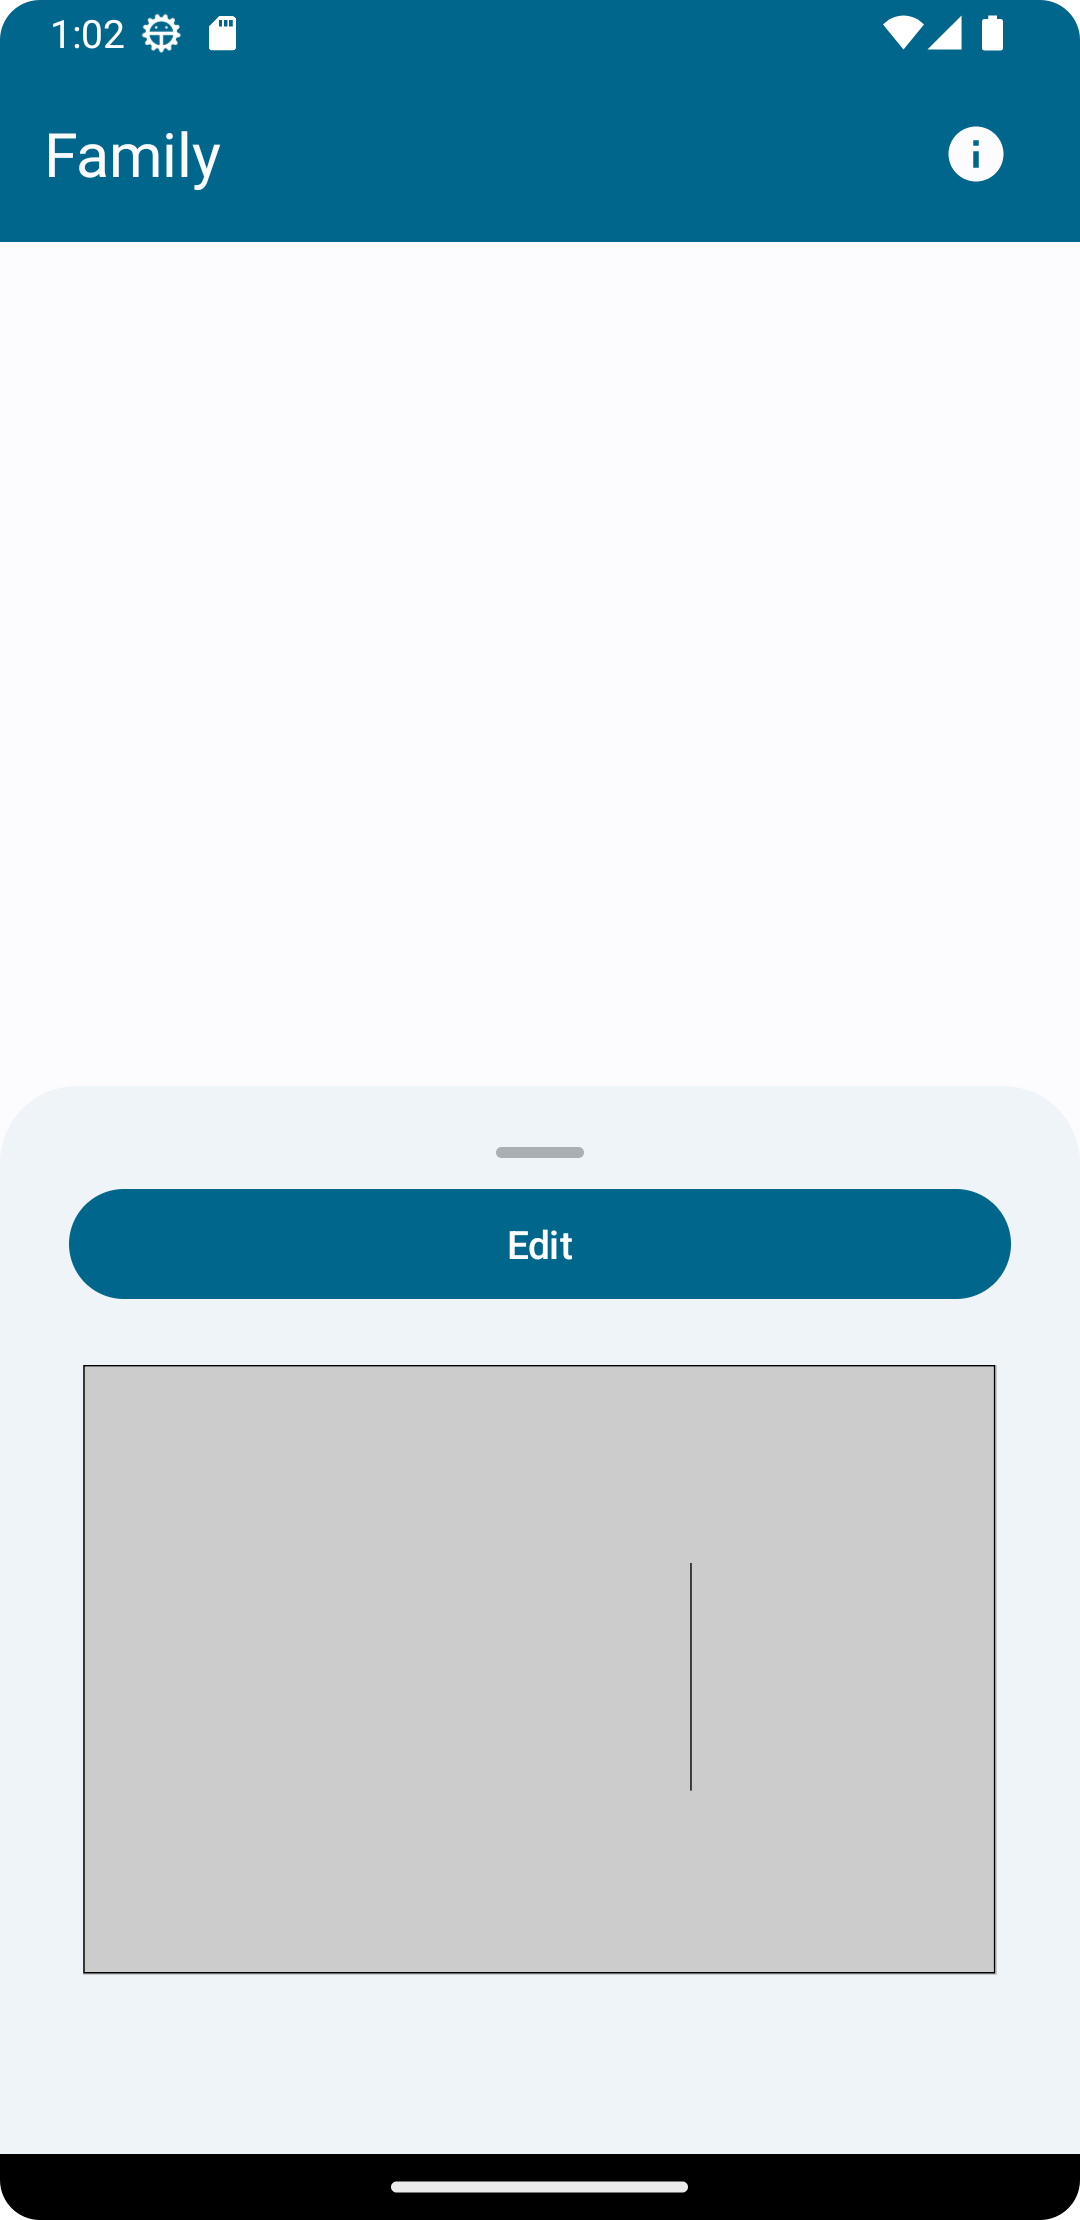
\includegraphics[trim={0cm -3cm 0 -3cm}, width=0.4\textwidth]{./Chapter6/Figures/ChatActivityPickPostcard}
	\caption{Chat Activity pick template}
	\label{fig:CVA3}
\end{figure}

On clicking the edit button the user is sent to the Draw Activity.

\begin{figure}[!ht]
	\centering
	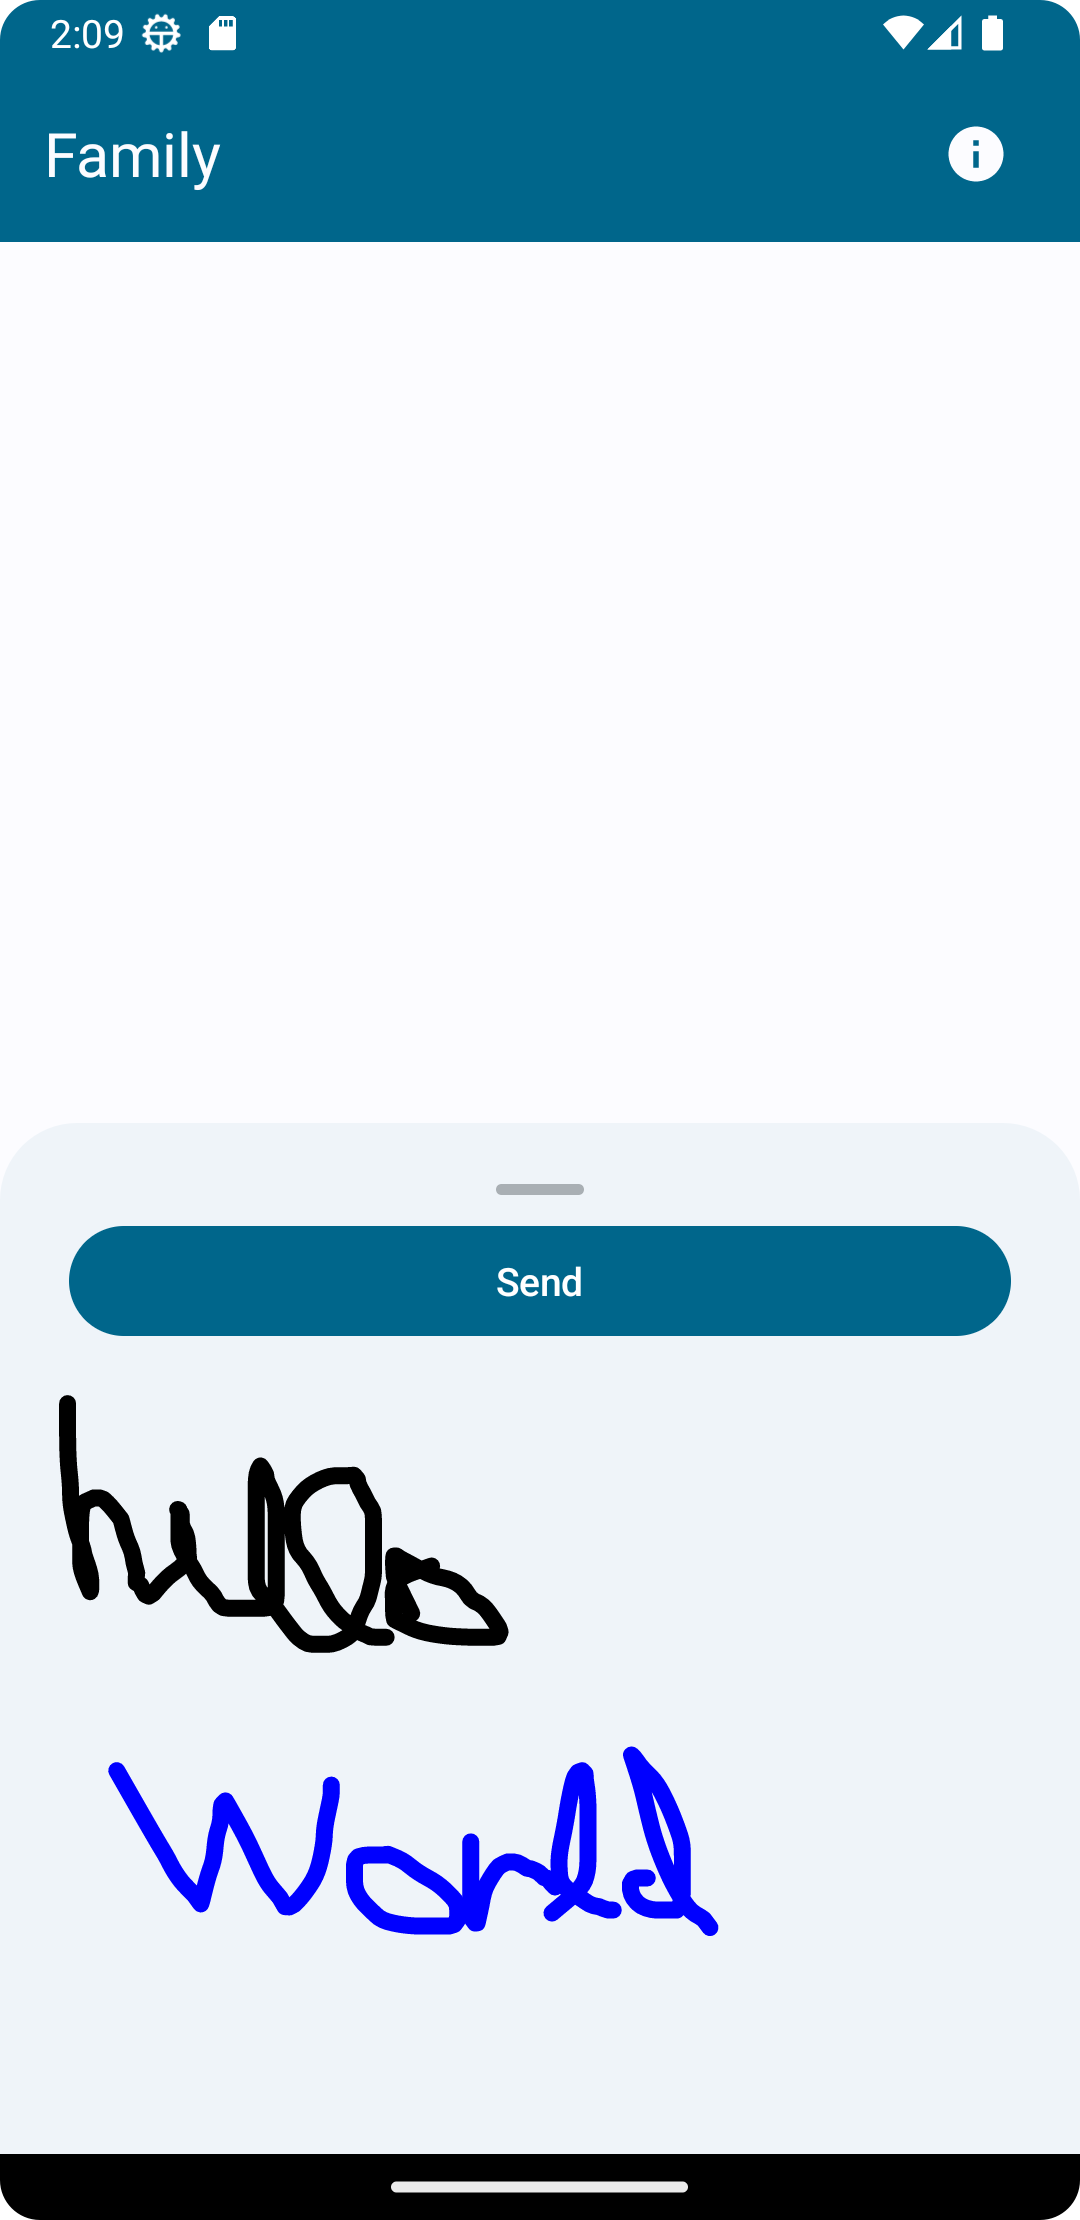
\includegraphics[trim={0cm -3cm 0 -3cm}, width=0.4\textwidth]{./Chapter6/Figures/ChatActivityPreview}
	\caption{CreateChat preview postcard}
	\label{fig:CVA4}
\end{figure}


\begin{figure}[!ht]
	\centering
	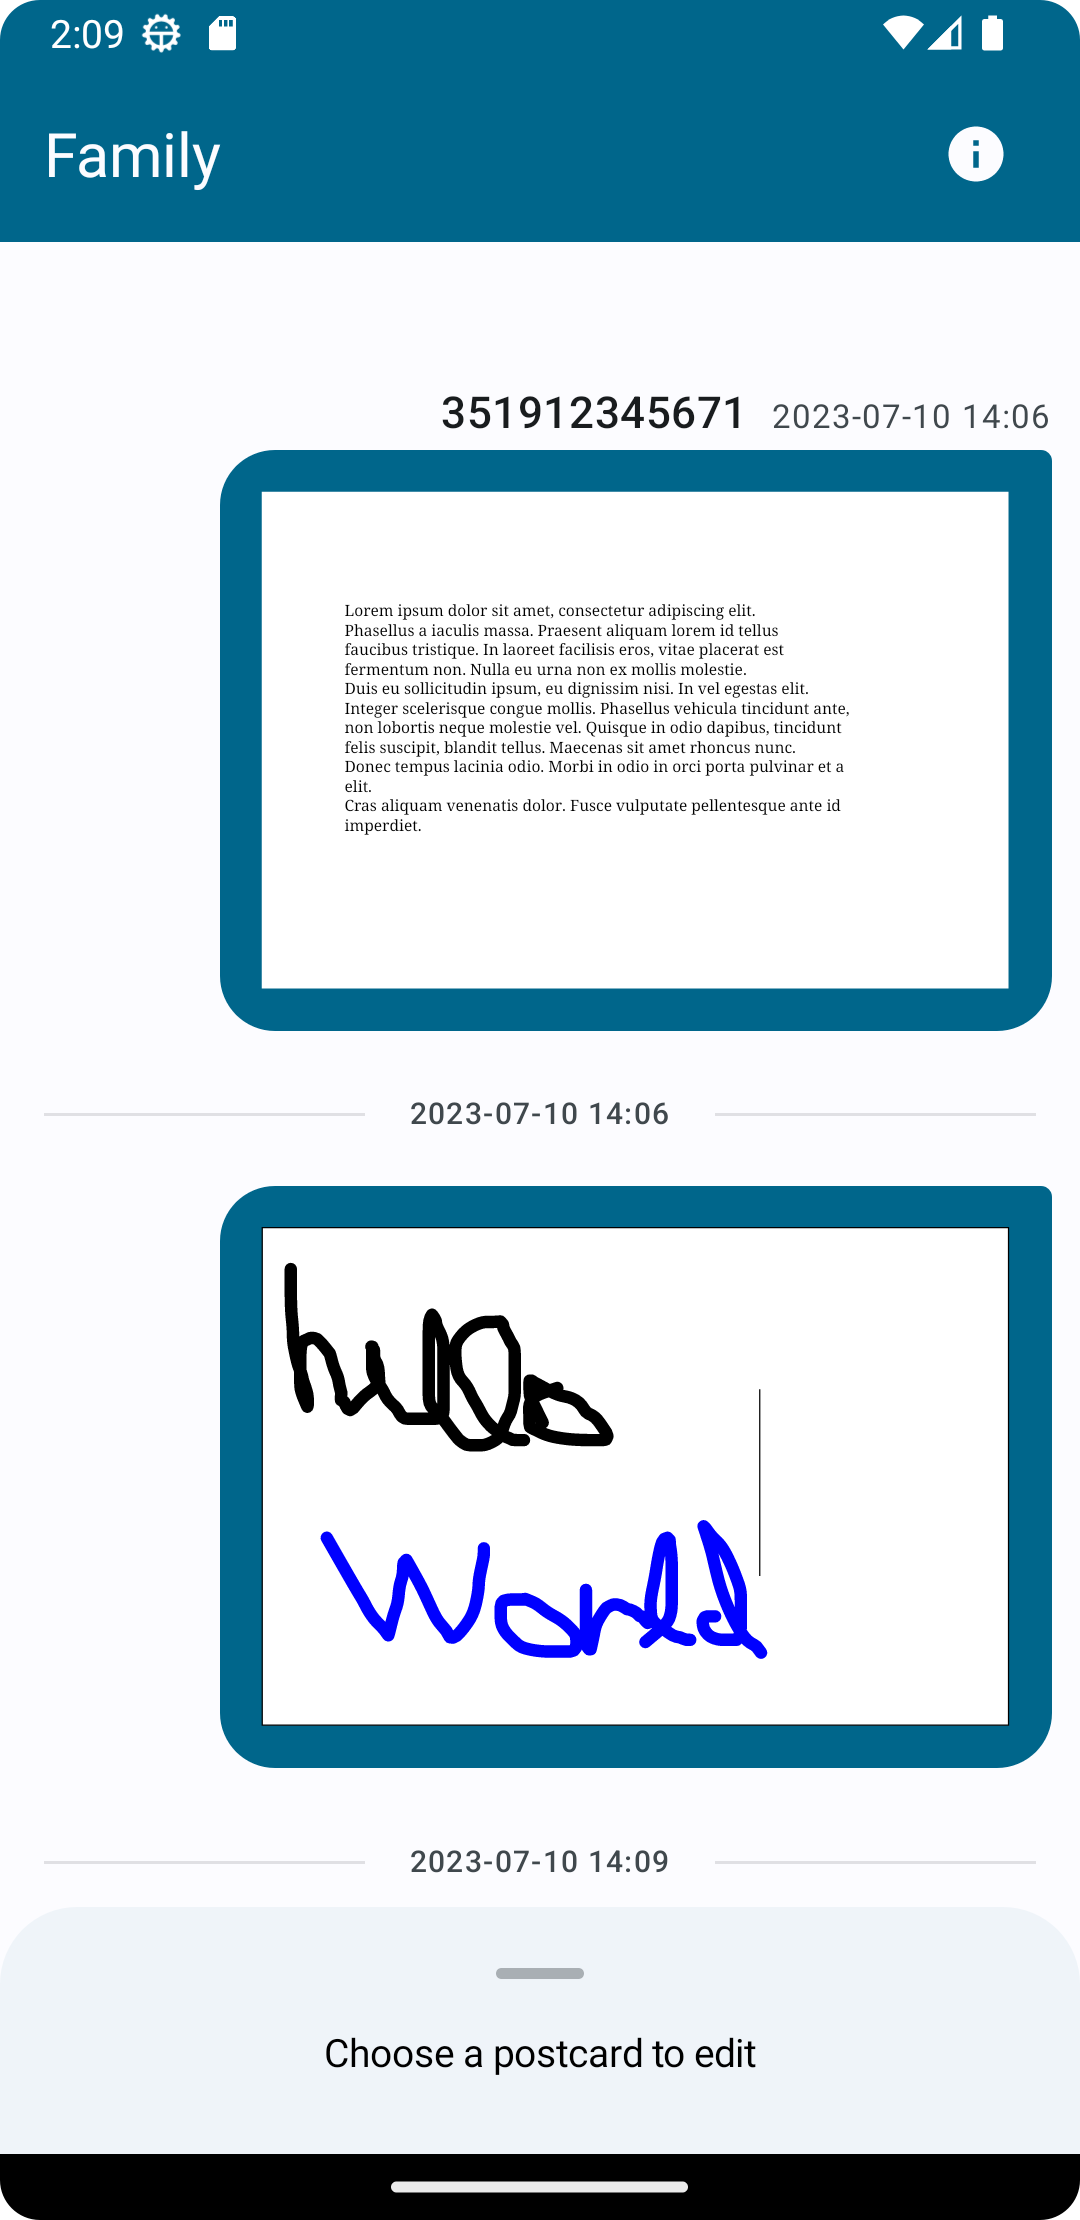
\includegraphics[trim={0cm -3cm 0 -3cm}, width=0.4\textwidth]{./Chapter6/Figures/ChatActivityUpdated}
	\caption{CreateChat postcard sent}
	\label{fig:CVA4}
\end{figure}



\subsection{Draw Postcard}
The Draw activity plays a crucial role in allowing users to edit and personalize a postcard using the Canvas. It involves implementing complex code to enable features such as drawing, zooming, and saving the postcard.

The challenge in implementing drawing and zoom features arise from the absence of a built-in two-finger zoom and one-finger touch draw function in the compose toolkit. To overcome this limitation, an in-depth analysis of the compose toolkit's inner code was conducted. By examining the underlying mechanisms of the compose toolkit, the necessary functionality for drawing and zooming was achieved.

To facilitate the saving of the canvas, a list is used to store the properties of each path. Each path property consists of the actual path data and the stroke style applied to it. When the canvas needs to be saved, the application iterates through each path in the list and generates an SVG file.

During the SVG file creation process, the application adds the necessary path movements and stroke styles to accurately represent each drawn path. This ensures that the saved SVG file faithfully represents the visual appearance of the canvas.

Figures \ref{fig:DA1} illustrate the implemented activity.



\begin{figure}[!ht]
	\centering
	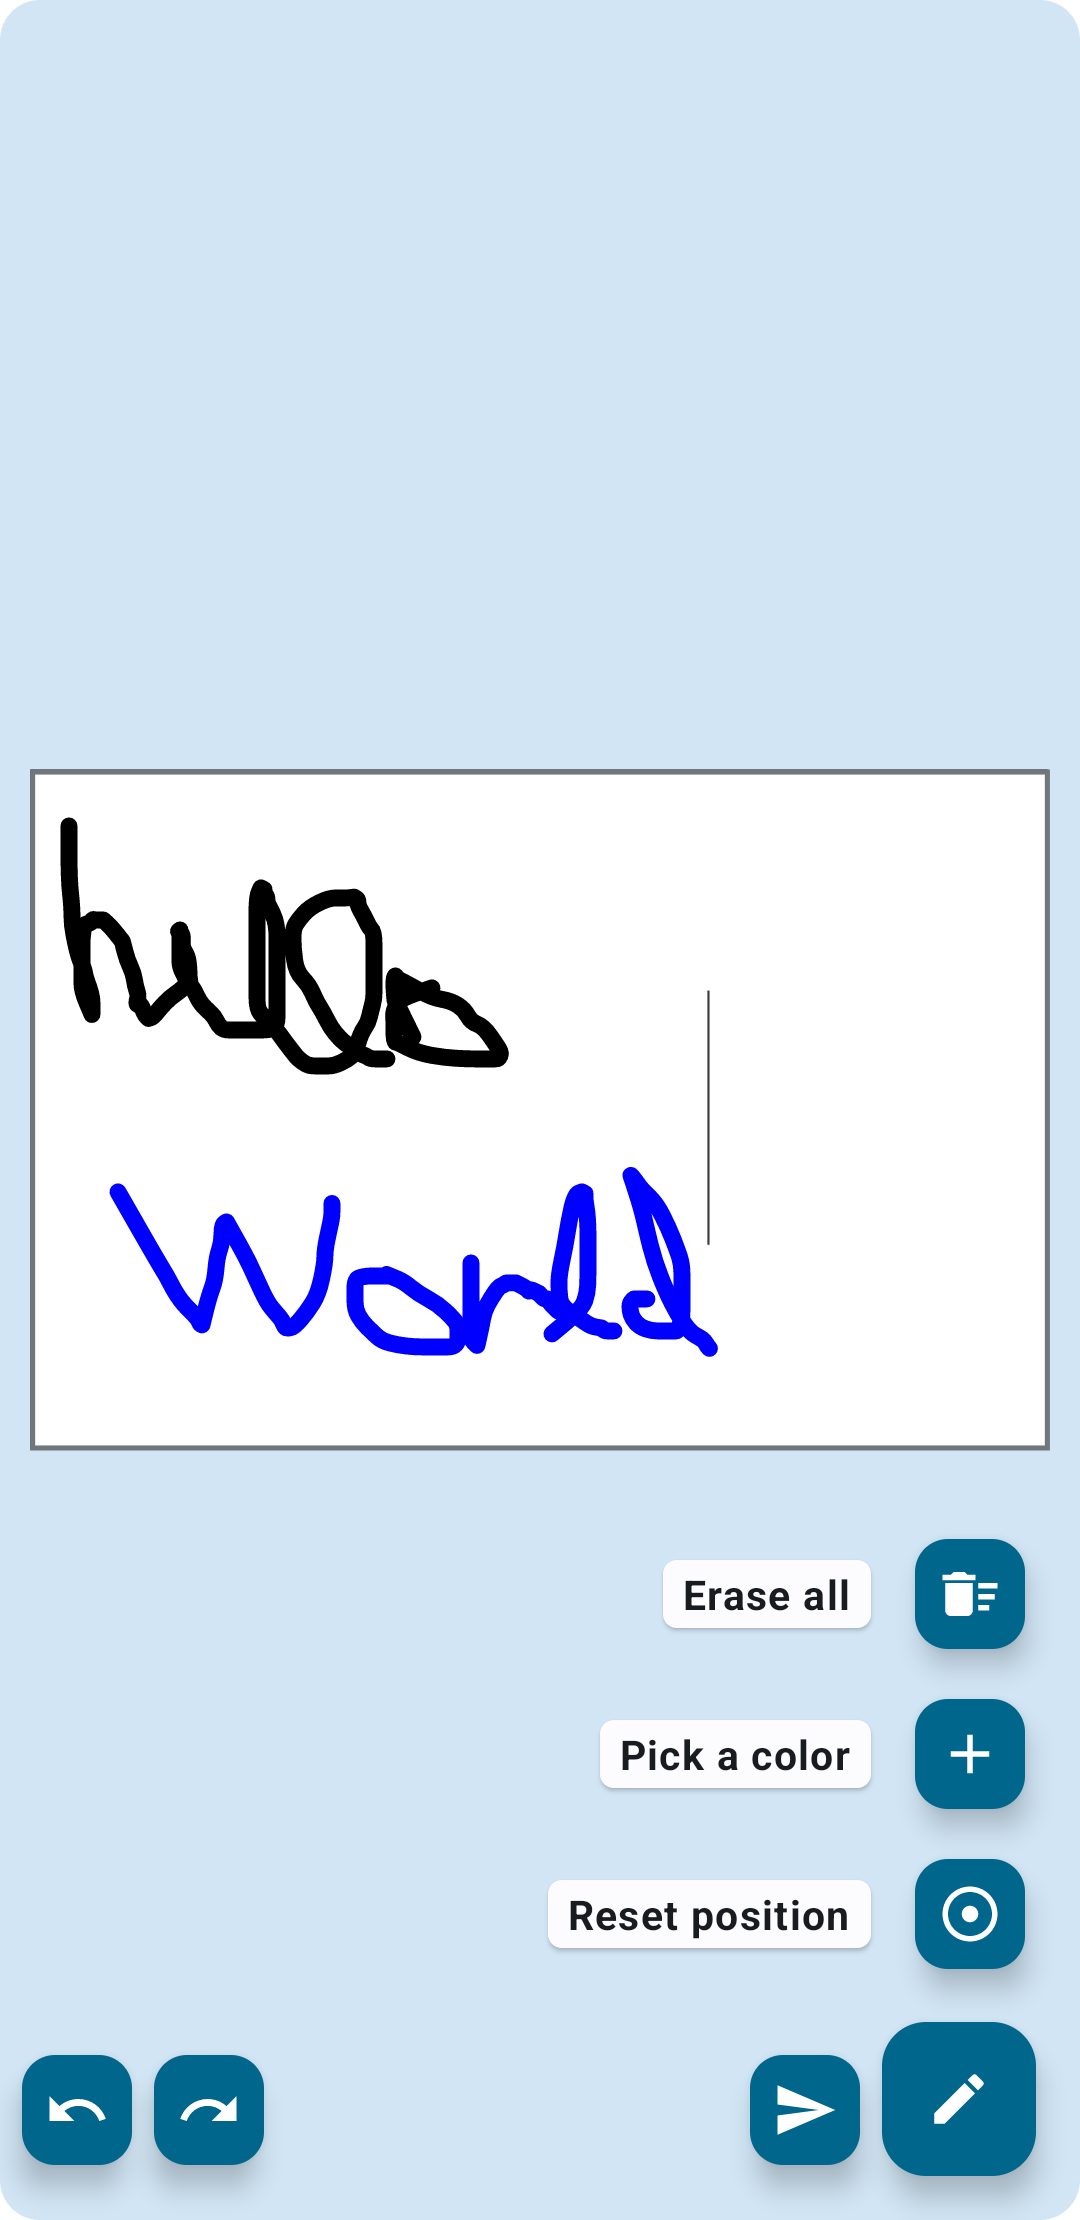
\includegraphics[trim={0cm -3cm 0 -3cm}, width=0.4\textwidth]{./Chapter6/Figures/DrawActivity}
	\caption{Draw Activity}
	\label{fig:DA1}
\end{figure}


\subsection{View Postcard}
The View Postcard Activity provides users with a dedicated interface to view postcards. It offers the ability to save and perform HTR over a postcard. 
When saving a file the user is prompted to choose the quality (from 1 to 5) this will multiply the default width and height of the SVG by the chosen value. The postcard is saved in the images media folder.
This activity focuses on delivering a seamless and immersive experience for users to enjoy the postcard content.

Figures \ref{fig:VA}, \ref{fig:VA1} and \ref{fig:VA2} illustrate the implemented activity.

\begin{figure}[!ht]
	\centering
	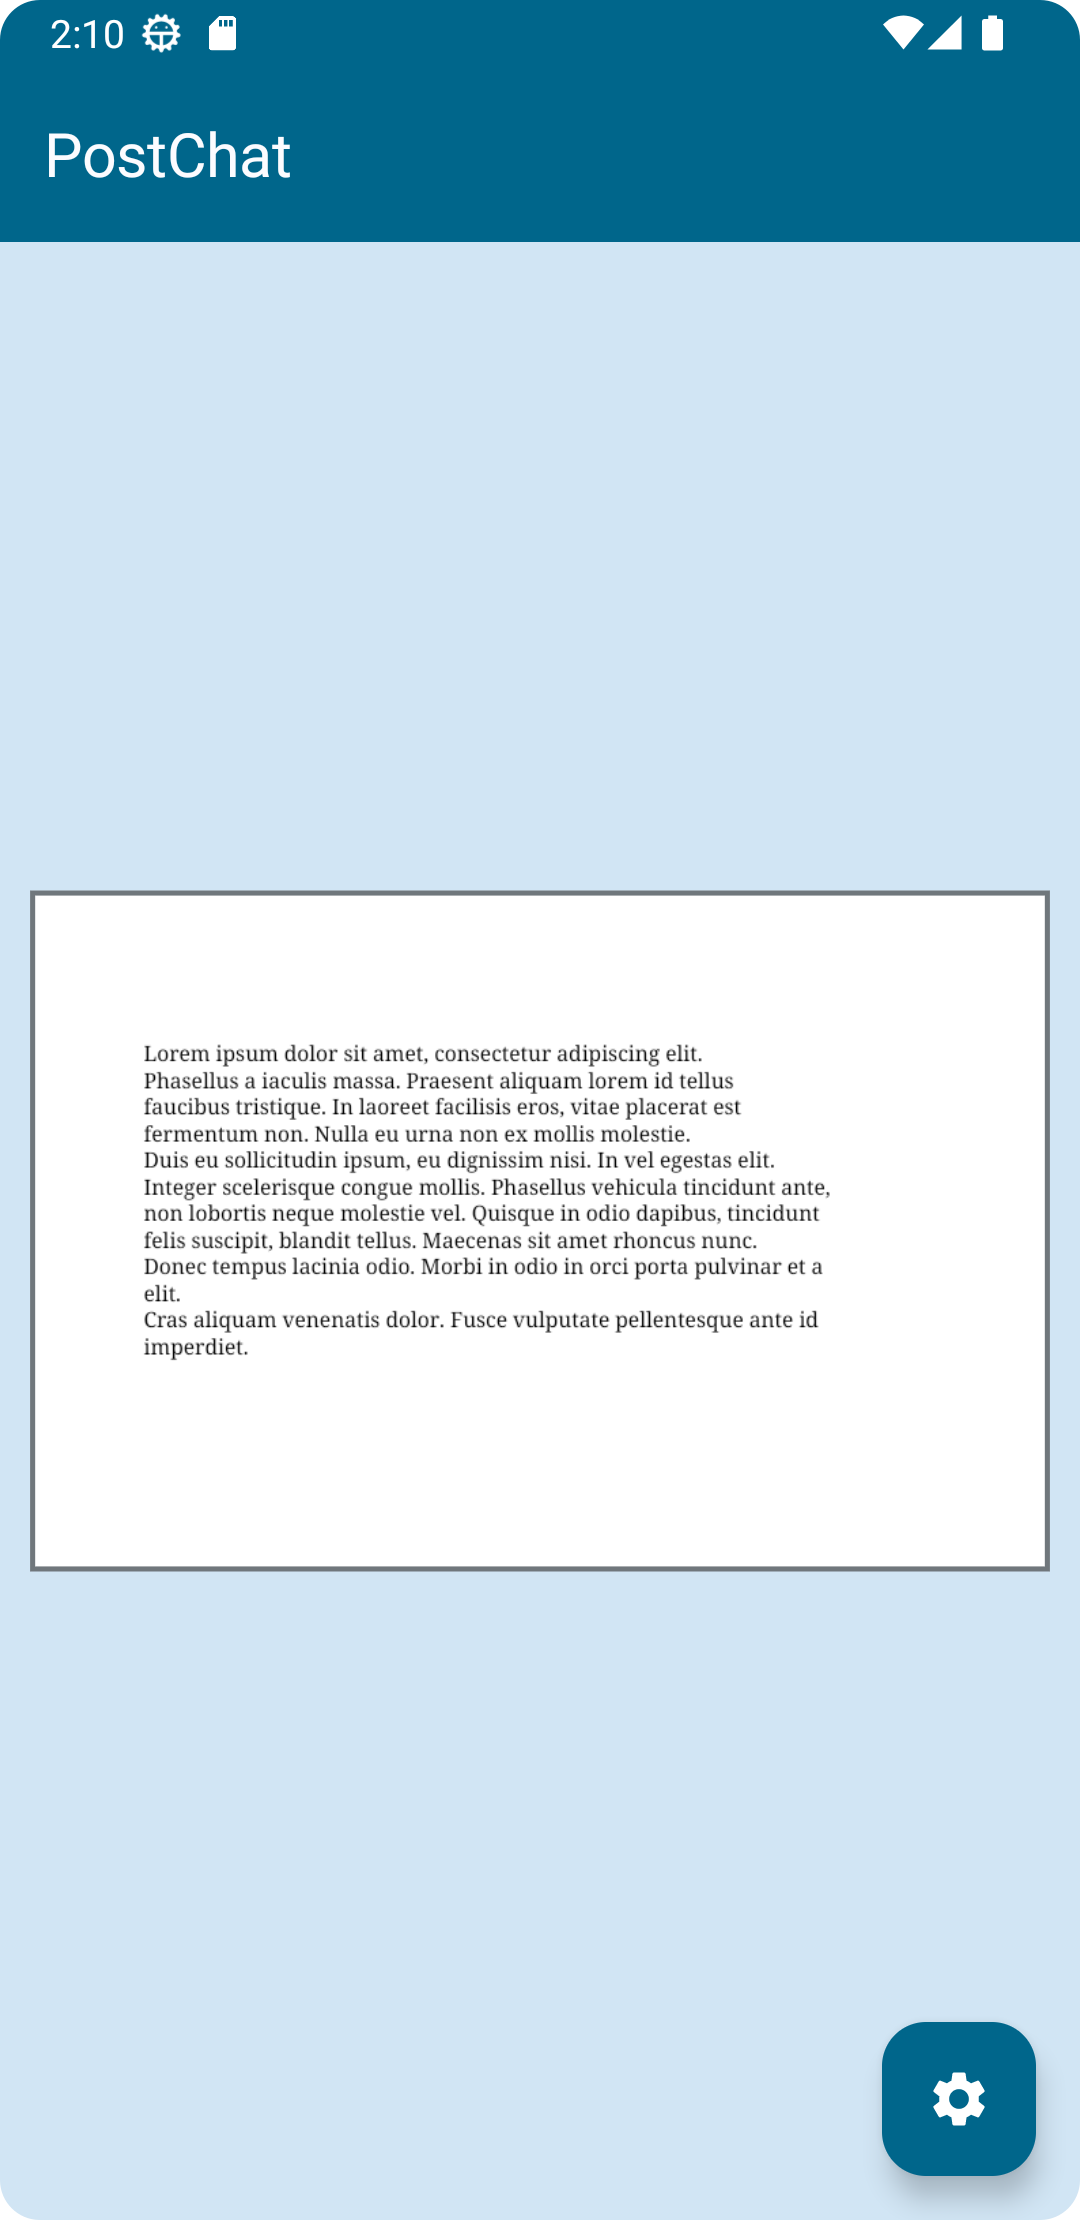
\includegraphics[trim={0cm -3cm 0 -3cm}, width=0.4\textwidth]{./Chapter6/Figures/PostcardActivity}
	\caption{Postcard View}
	\label{fig:VA}
\end{figure}


\begin{figure}[!ht]
	\centering
	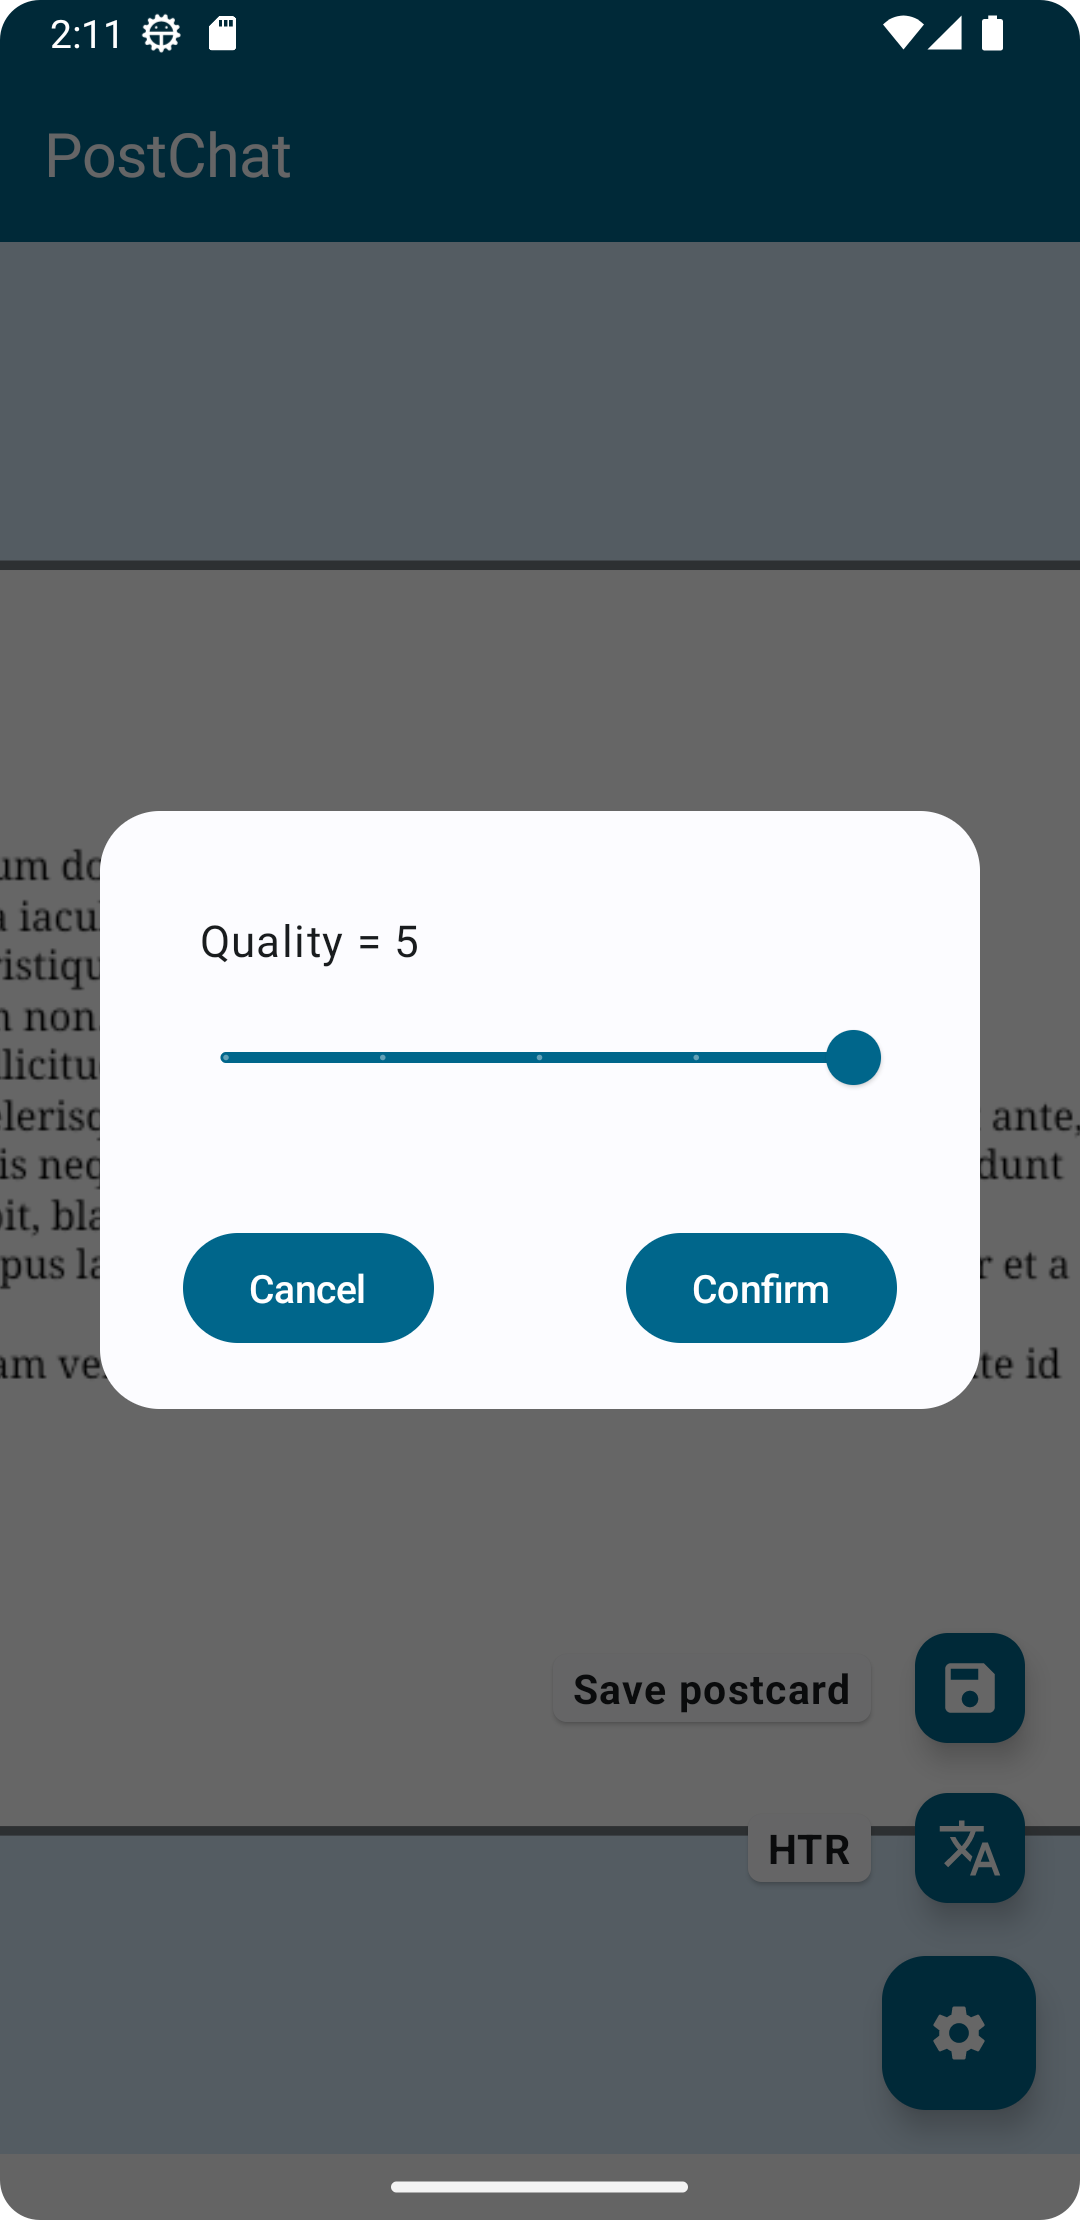
\includegraphics[trim={0cm -3cm 0 -3cm}, width=0.4\textwidth]{./Chapter6/Figures/PostcardActivitySave}
	\caption{Postcard save}
	\label{fig:VA1}
\end{figure}

\begin{figure}[!ht]
	\centering
	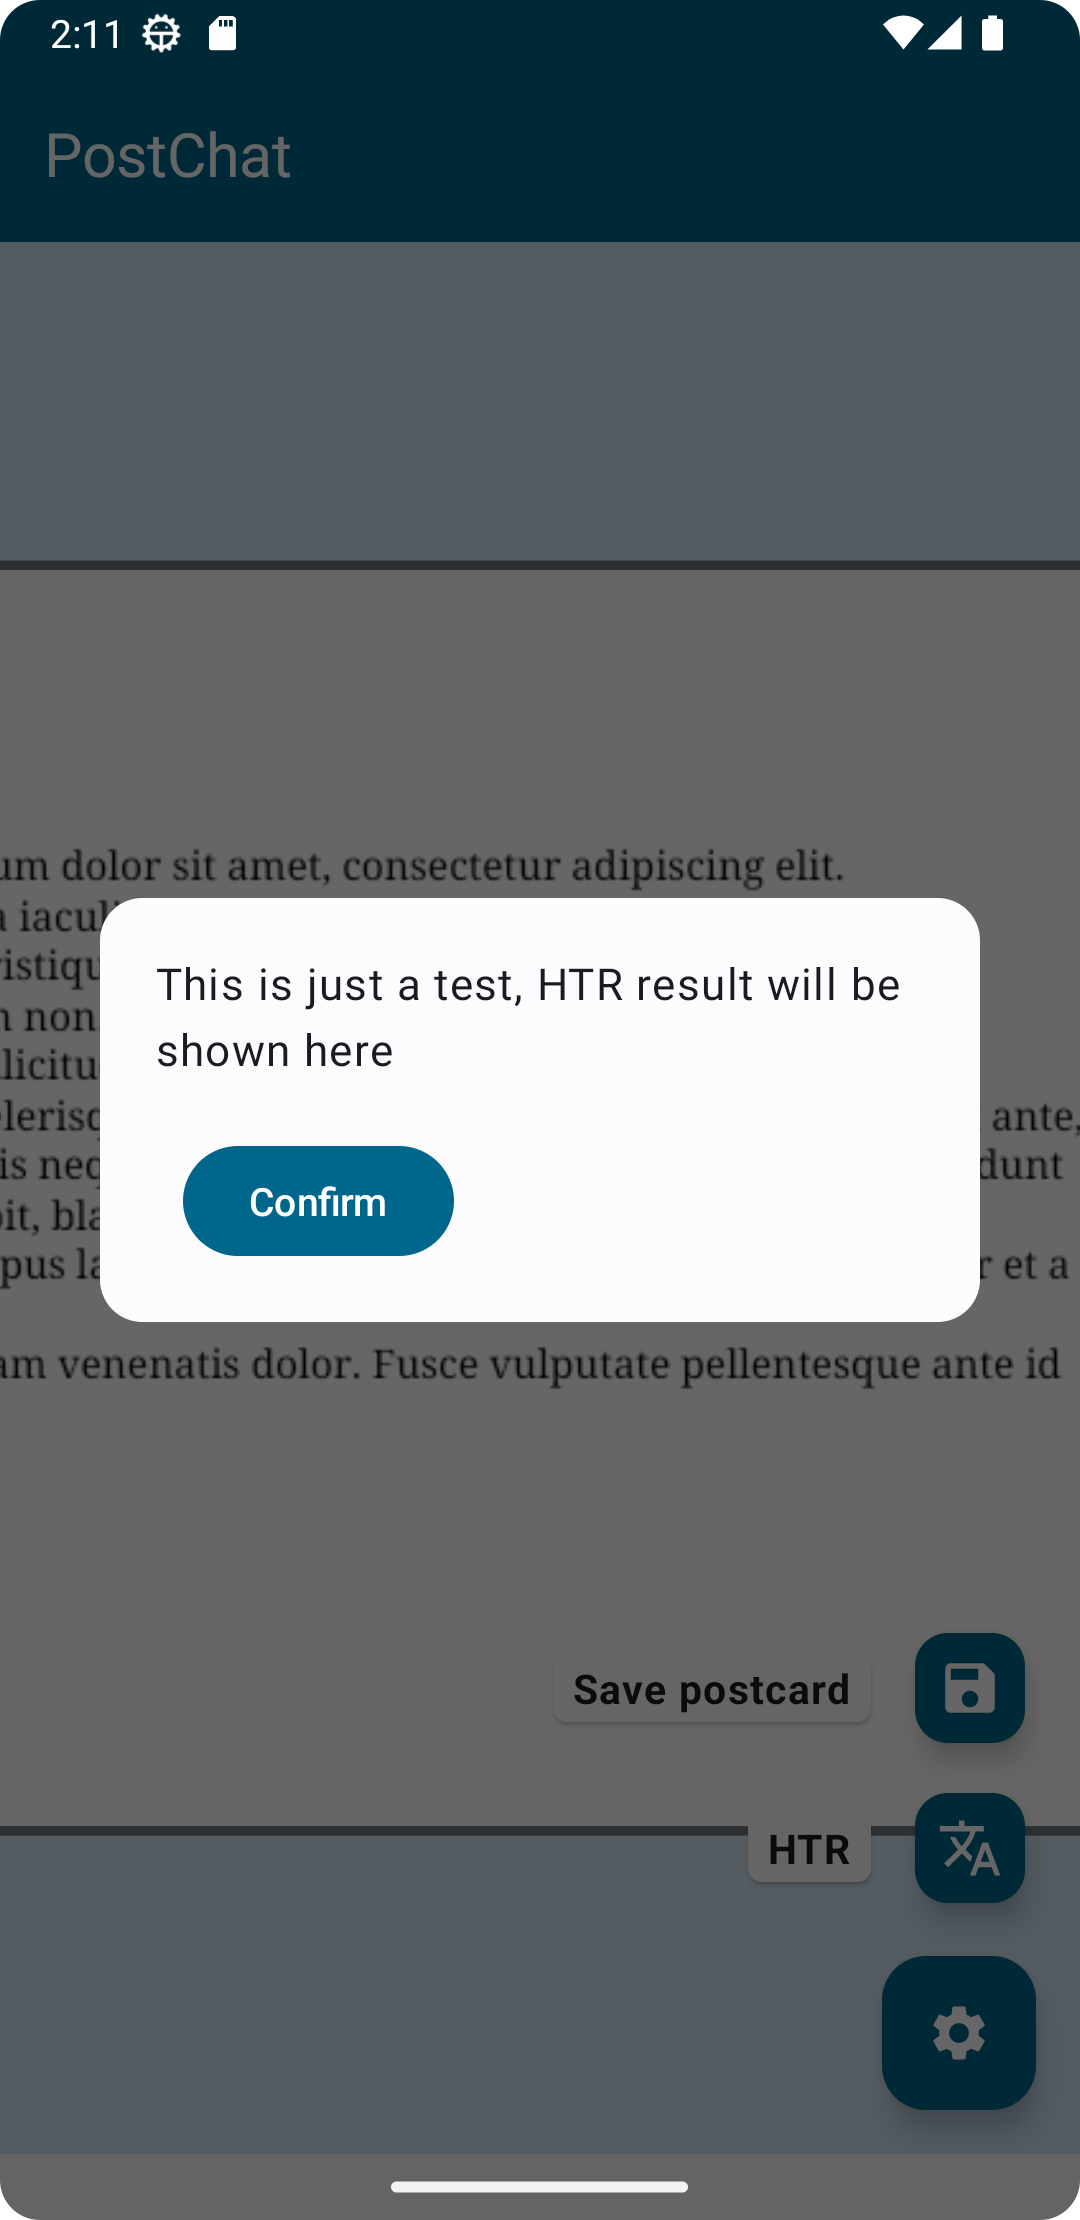
\includegraphics[trim={0cm -3cm 0 -3cm}, width=0.4\textwidth]{./Chapter6/Figures/PostcardActivityHTR}
	\caption{Postcard perform HTR}
	\label{fig:VA2}
\end{figure}


\subsection{Settings and Information}
The settings activity plays a major role in debugging but it is not limited to just that.

In this activity a user can delete its account or logout from the service.
Other settings are just for data visualization by the programmer and should be treated as so. They offer no utility for the final consumer and will be hidden from the same when ready for production.

There is a icon in the top right of the corner that leads to the activity containing information about the program and team behind it.

Figures \ref{fig:SIA} and \ref{fig:SIA1} illustrate the implemented activities.

\begin{figure}[!ht]
	\centering
	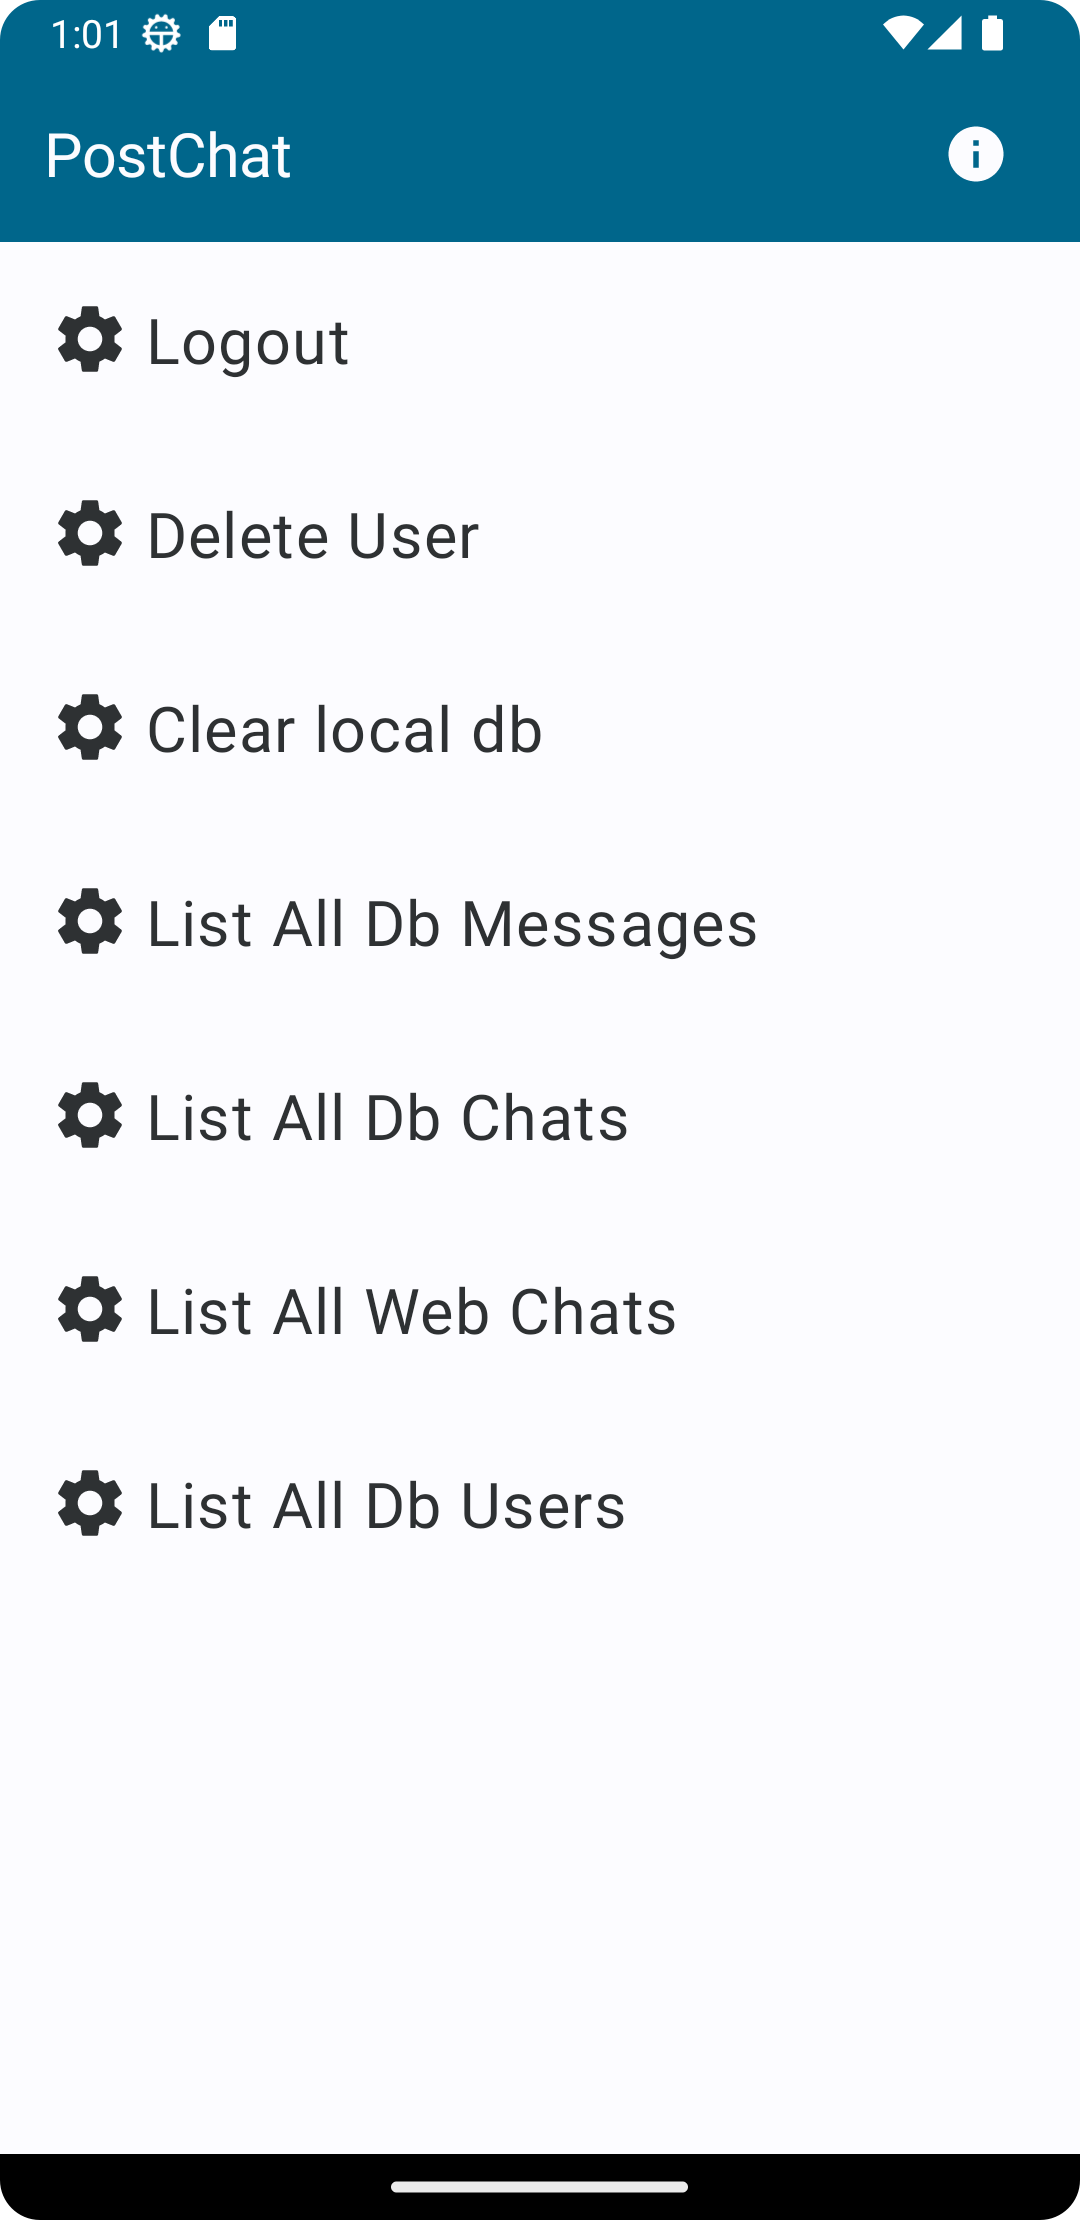
\includegraphics[trim={0cm -3cm 0 -3cm}, width=0.4\textwidth]{./Chapter6/Figures/SettingsActivity}
	\caption{Settings activity}
	\label{fig:SAI}
\end{figure}


\begin{figure}[!ht]
	\centering
	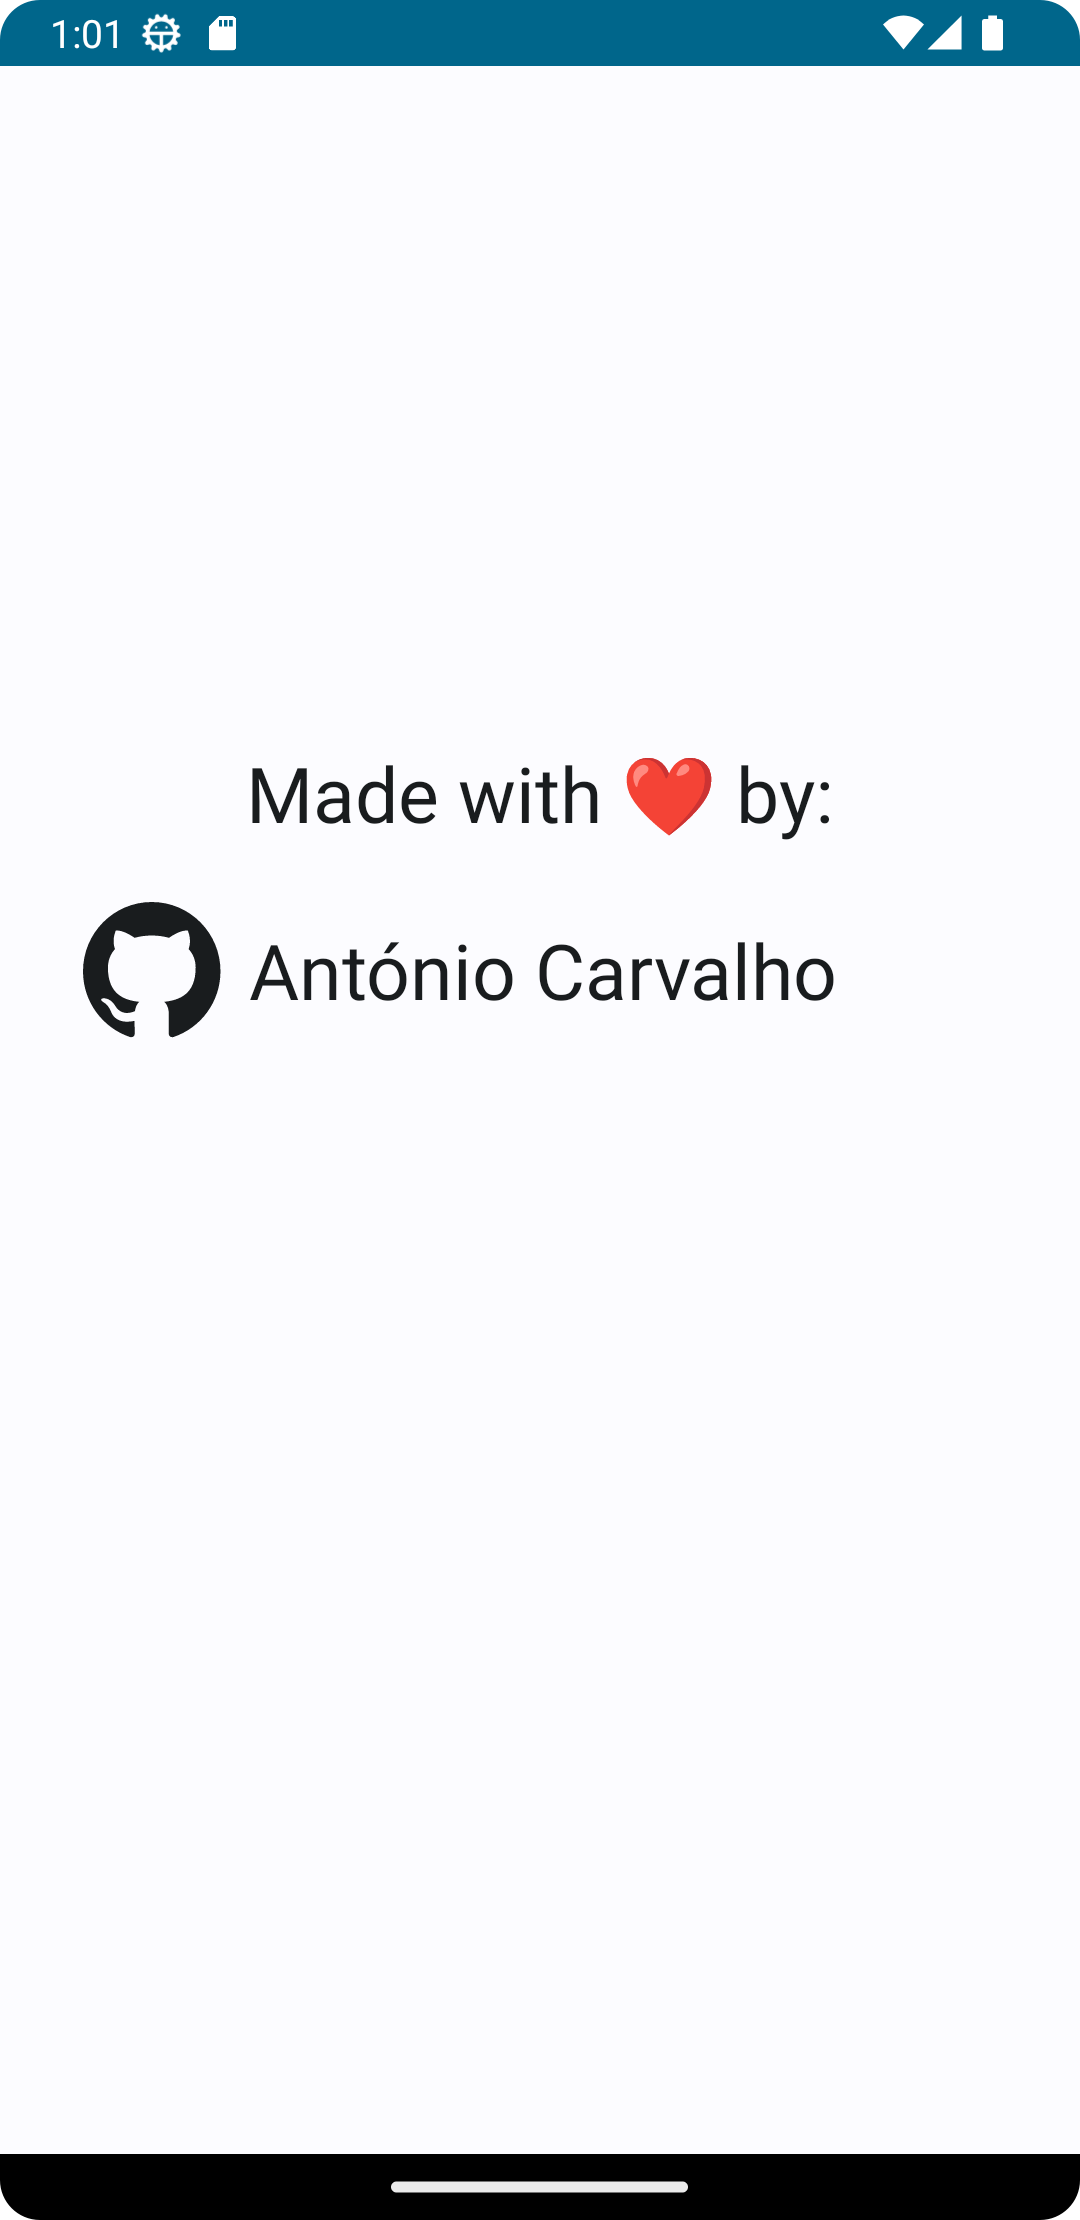
\includegraphics[trim={0cm -3cm 0 -3cm}, width=0.4\textwidth]{./Chapter6/Figures/InfoActivity}
	\caption{Information activity}
	\label{fig:SAI1}
\end{figure}


